\documentclass[12pt]{article} 
\usepackage[letterpaper, margin=2.5cm]{geometry}
% enlaza la tabla de contenido con las paginas
\usepackage[linktoc=all ]{hyperref}
% usar con XETEX
\usepackage{fontspec} % quite [no-math] si presenta error en compilacion
\setmainfont{Times New Roman}
\setlength{\parindent}{1.2cm} % sangria de 1.2cm en la primera linea del parrafo
%\usepackage[utf8]{inputenc} 

%%%%%%%%%%%%%%%%%%%%%%%%%%%%%%%%%%%%%%%%%%%%%%
%%%% evita que coloque guiones al justificar
%%%%%%%%%%%%%%%%%%%%%%%%%%%%%%%%%%%%%%%%%%%%%%
  %\tolerance 9999
  %\emergencystretch 3em
  %\vfuzz\hfuzz

% https://sumanta679.wordpress.com/2009/05/20/latex-justify-without-hyphenation/
\tolerance=1000
\emergencystretch=\maxdimen
\hyphenpenalty=10000
\hbadness=10000

%\usepackage{hyphenat}
%\usepackage{microtype}
%\usepackage[none]{hyphenat}

%\tolerance=9999
%\emergencystretch=10pt
%\hyphenpenalty=10000
%\exhyphenpenalty=100


%%%%%%%%%%%%%%%%%%%%%%%%%%%%%%%%%%%%%%
%        interlineado 1.5
%%%%%%%%%%%%%%%%%%%%%%%%%%%%%%%%%%%%%%
%─────────────────────────────────────┐
\usepackage{setspace}                %│  
\onehalfspacing                      %│
%─────────────────────────────────────┘

%%%%%%%%%%%%%%%%%%%%%%%%%%%%%%%%%%%%%%
%  elimina identacion en las listas
%  se usa el paquete enumitem
%%%%%%%%%%%%%%%%%%%%%%%%%%%%%%%%%%%%%%
%─────────────────────────────────────┐
\usepackage{enumitem}                %│          
\setlist[itemize]{leftmargin=*}      %│  
%─────────────────────────────────────┘

%%%%%%%%%%%%%%%%%%%%%%%%%%%%%%%%%%
% paquete para referencias
%%%%%%%%%%%%%%%%%%%%%%%%%%%%%%%%%%
\usepackage[style=ieee]{biblatex}
\addbibresource{bibs/sample.bib}   



% para que las urls tengan la misma fuente que resto del documento
%https://tex.stackexchange.com/questions/106622/how-to-change-the-font-of-url-in-the-bibliography
\usepackage{url}
\urlstyle{same}

%% coloca s.f cuando no tiene anio la referencia
%% https://copyprogramming.com/howto/biblatex-and-entries-with-no-date
%\newcommand{\mkbibnodate}{s\adddot f\adddot}
%\AtEveryCitekey{\iffieldundef{labelyear}{\restorefield{labelyear}{\mkbibnodate}}{}}
%\AtEveryBibitem{\iffieldundef{labelyear}{\restorefield{year}{\mkbibnodate}}{}}

% https://tex.stackexchange.com/questions/612417/biblatex-and-entries-with-no-date-part-2
\renewbibmacro*{date}{%
  \iffieldundef{year}
    {\bibstring{nodate}}
    {\printdate}}

\DeclareFieldFormat{url}{[Internet]\adddot\space\bibstring{urlfrom}\space\url{#1}}

\DeclareFieldFormat{urldate}{\adddot\addspace[\bibstring{urlseen}\addcolon\space #1]}

% puntos en cada entrada d la biliografia
\renewcommand*{\newunitpunct}{\addcomma\space}
%\renewcommand*{\newunitpunct}{\addperiod\space}
  
\DefineBibliographyStrings{spanish}{%
  urlfrom = {Disponible en},
  urlseen = {Consultado}
} 


\newbibmacro*{author+title+date}{%
  \ifnameundef{editor}
    {}
    {%
      \usebibmacro{editor}%
      \setunit{\addspace}%
      \printnames[byeditor]{editor}%
      \clearname{editor}%
      \newunit
    }%
  \usebibmacro{byeditorx}%
  \usebibmacro{bytranslator+others}%
  \ifnameundef{author}
  {%
    \printfield{title}
    \printtext[parens]{\usebibmacro{date}}
  }%
  {%
      \usebibmacro{author}\addcomma\space%
      \printtext[parens]{\usebibmacro{date}} \adddot \addspace %
      \printfield{title} \adddot
  }%
}



\DeclareBibliographyDriver{online}{%
  \usebibmacro{bibindex}%
  \usebibmacro{begentry}%
  %\usebibmacro{author/editor+others/translator+others}%
  \usebibmacro{author+title+date}%
  %\setunit{\adddot\addspace}% ELIMINADO
  %\usebibmacro{title}%        ELIMINADO  
  \setunit{\adddot\addspace}%
  \printlist{language}%
  \setunit{\adddot\addspace}%
  \usebibmacro{byauthor}%
  \setunit{\adddot\addspace}%
  \usebibmacro{byeditor+others}%
  \setunit{\adddot\addspace}%
  \printfield{version}%
  \setunit{\adddot\addspace}%
  \printfield{note}%
  \newunit\newblock
  \printlist{organization}%
  \setunit{\adddot\addspace}%
  \iftoggle{bbx:eprint}
    {\usebibmacro{eprint}}
    {}%
  \setunit{\adddot\addspace}%
  %\printtext[parens]{\usebibmacro{date}}% ELIMINDADO
  %\newunit\newblock                     % ELIMINDADO
  \usebibmacro{url+urldate}%
  \setunit{\adddot\addspace}%
  \usebibmacro{addendum+pubstate}%
  \setunit{\bibpagerefpunct}\newblock
  \usebibmacro{pageref}%
  \newunit\newblock
  \iftoggle{bbx:related}
    {\usebibmacro{related:init}%
     \usebibmacro{related}}
    {}%
  \usebibmacro{finentry}}



%\usepackage{showframe}% http://ctan.org/pkg/showframe

% paquete para los encabezados
\usepackage{fancyhdr}
\usepackage{xcolor}
% tabla de contenido
% la opcion titles evita que sobreescriba 
% los encabezados de fancyhdr.
\usepackage[titles]{tocloft}

\usepackage{layout}

% cambia las secciones y afecta al paquete hyperref en la tabla de contenido
% agregar \phantomsection a cada adicion manual a la tabla de contenido
% incluyenndo la bibliografia para que el anchor ref sea correcto
\usepackage{titlesec} 

\usepackage{indentfirst}
\usepackage{newtxtext}
\usepackage{blindtext}
%\usepackage{showframe}

% tablas
\usepackage{tabularx, ragged2e, longtable, xltabular} 
\usepackage{colortbl}
\usepackage{graphicx}
\usepackage{tikz}
\usetikzlibrary{shapes.geometric, arrows.meta, positioning, fit, backgrounds, calc}


\usepackage{mwe}
\usepackage{graphbox} %loads graphicx package
\usepackage{makecell}
% paquetes para tablas
\usepackage{booktabs}

\usepackage{multirow}
% paquete para codigo
\usepackage{minted} 
% se usa babel para cambiar a español las referencias
% (fechas (Jan->ene), páginas(pp->págs.),etc)
\usepackage[spanish, english]{babel}

\usepackage{csquotes}
\usepackage{amsmath}
\usepackage{amssymb}
\usepackage{caption}
\usepackage{float}

% alinear figuras
\usepackage[export]{adjustbox}

%%%%%% paquetes eliminados %%%%%%
%\usepackage{array}


\renewcommand{\cftpartleader}{\cftdotfill{\cftdotsep}} % for parts
\renewcommand{\cftsecleader}{\cftdotfill{\cftdotsep}} % for sections, if you really want! (It is default in report and book class (So you may not need it).

%centra la tabla de figuras
\renewcommand{\cftloftitlefont}{\hspace*{\fill}\Huge\bfseries}
\renewcommand{\cftafterloftitle}{\hspace*{\fill}}
% centra la lista de tablas
\renewcommand{\cftlottitlefont}{\hspace*{\fill}\Huge\bfseries}
\renewcommand{\cftafterlottitle}{\hspace*{\fill}}
% centra la lista de tablas
\renewcommand{\cfttoctitlefont}{\hspace*{\fill}\Huge\bfseries}
\renewcommand{\cftaftertoctitle}{\hspace*{\fill}}

\setcounter{tocdepth}{5}
\setlength{\cftsecindent}{0pt}% Remove indent for \section
\setlength{\cftsubsecindent}{1.5em}% Remove indent for \subsection
\setlength{\cftsubsubsecindent}{2.0em}% Remove indent for \subsubsection
\setlength{\cftparaindent}{2.5em}% Remove indent for \paragraph
\setlength{\cftsubparaindent}{3.0em}% Remove indent for \subparagraph

\setlength{\cftsecnumwidth}{3.0em}
\setlength{\cftsubsecnumwidth}{1.5em}% Remove numwidth for \subsection
\setlength{\cftsubsubsecnumwidth}{2.0em}% Remove numwidth for \subsubsection
\setlength{\cftparanumwidth}{1.5em}% Remove numwidth for \paragraph
\setlength{\cftsubparanumwidth}{1.5em}% Remove numwidth for \subparagraph




%%%%%%%%%%%%%%%%%%%%%%%%%%%%%
%  usa el paquete titlesec
%%%%%%%%%%%%%%%%%%%%%%%%%%%%

% Centrar títulos de secciones
%\usepackage{sectsty}
%\sectionfont{\centering}

% Empezar sección en una nueva pagina
\let\stdsection\section
\renewcommand\section{\cleardoublepage\stdsection}

%  formato aplicado en la tabla de contenido 
\renewcommand{\thesection}{\Roman{section}}
\renewcommand{\thesubsection}{\Alph{subsection}}
\renewcommand{\thesubsubsection}{\arabic{subsubsection})}
\renewcommand{\theparagraph}{\alph{paragraph})}

% paquete titlesec
\titleformat{\section}[hang]
    {\filcenter\normalfont\normalsize\bfseries} % centra la seccion 
    {\Roman{section}.}
    {1em}{}[]

% paquete titlesec
\titleformat{\subsection}[hang]
    {\normalfont\normalsize\bfseries}     % la subseccion ya esta centrada por defecto
    {\Alph{subsection}.}
    {1em}{}

% paquete titlesec
\titleformat{\subsubsection}[runin]{\normalfont\itshape\normalsize\bfseries}
    {\arabic{subsubsection})}
    {1em}
    {}
    [:]
\titlespacing{\subsubsection}{0.5cm}{*1}{*1}[0cm]

% paquete titlesec
\titleformat{\paragraph}[runin]{\normalfont\itshape\normalsize\bfseries}
    {\alph{paragraph})}
    {1em}
    {}
    [:]
\titlespacing{\paragraph}{1.0cm}{*1}{*1}[0cm]

\newcommand{\shortlorem}{Lorem ipsum dolor sit amet, consectetuer adipiscing elit. Etiam lobortis facilisis sem. Nullam
nec mi et neque pharetra sollicitudin. Praesent imperdiet mi nec ante.}

% usa pakage caption
\renewcommand{\thetable}{\Roman{table}}
\captionsetup[table]{labelfont=bf, labelsep=newline}
\captionsetup[figure]{labelfont=bf, labelsep=period}

%%%%%%%%%%%%%%%%%%%%%%%%%%%%%%%%%%%%%%%%%%%%%%%%%%%%%%
%        key words - palabras clave
%%%%%%%%%%%%%%%%%%%%%%%%%%%%%%%%%%%%%%%%%%%%%%%%%%%%%%
\providecommand{\keywords}[1]
{
  \small	
  \textbf{\textit{Keywords --- } #1 } 
  %%%%%%%%%%%%%%%%%%%%%%%%%%%%%%%%%%%%
  %  regresa la fuente a 12 pt
  %%%%%%%%%%%%%%%%%%%%%%%%%%%%%%%%%%%%
 \normalsize
}

\providecommand{\palabrasclave}[1]
{
  \small	
  \textbf{\textit{Palabras clave --- } #1 } 
  %%%%%%%%%%%%%%%%%%%%%%%%%%%%%%%%%%%%
  %  regresa la fuente a 12 pt
  %%%%%%%%%%%%%%%%%%%%%%%%%%%%%%%%%%%%
 \normalsize
}



%usa package array
% nuevo tipo de columna (P mayuscula) que centra el texto
\newcolumntype{P}[1]{>{\centering\arraybackslash}p{#1}}


% usa pakage babel y cquotes
\addto\captionsenglish{\renewcommand{\contentsname}{TABLA DE CONTENIDO}}
\addto\captionsenglish{\renewcommand{\listfigurename}{LISTA DE FIGURAS}}
\addto\captionsenglish{\renewcommand{\listtablename}{LISTA DE TABLAS}}
\addto\captionsenglish{\renewcommand{\figurename}{Fig.}}
\addto\captionsenglish{\renewcommand{\tablename}{TABLA}}


\title{Plantilla}
\author{Author Name }
\date{May 2022}


%%%%%%%%%%%%%%%%%%%%%%%%%%%%%%%%%%
%        eliminados 
%%%%%%%%%%%%%%%%%%%%%%%%%%%%%%%%%%%

%usa package makecell
%usado en config/pages/tables/tabla_como_citar
%\newlist{mylist}{enumerate}{2}% a new list named: mylist, of type: enumerate, with number of levels: 2

%\setlist[mylist,1]{leftmargin=0.6cm,label={\alph*)}, topsep=0pt}% defining the first level
%\setlist[mylist,2]{leftmargin=1cm,label={\roman*)}}% defining the second level 

\newcommand{\celdauno}{}
\newcommand{\celdados}{}
\newcommand{\celdatre}{}
\newcommand{\celdacua}{}
\newcommand{\celdacin}{}
\newcommand{\celdasei}{}
\newcommand{\celdasie}{}
\newcommand{\celdaoch}{}
\newcommand{\celdanue}{}

\newcommand{\autoresportada}{
Julian Gómez Posada 
}

\newcommand{\autorescitacion}{
J. Gómez Posada
}

\newcommand{\autorescitaciontexto}{
Gonzáles Mejía et al
}

\newcommand{\titulo}{Sistema de mitigación de accidentes de tránsito para ciudad con grandes urbes: Caso Medellín}

\newcommand{\tituloencabezado}{Sistema de mitigación de accidentes de tránsito para ciudad con grandes urbes: Caso Medellín}

\newcommand{\tipodocumento}{
Trabajo de Grado presentado
%Anteproyecto presentado
}

\newcommand{\tituloporoptar}{
Ing. Datos y software
%Administrador de empresas
}

%%%%%%%%%%%%%%%%%%%%%%%%%%%%%%%%%%%%%%%
%           Asesor o asesores 
%%%%%%%%%%%%%%%%%%%%%%%%%%%%%%%%%%%%%%%

% si es un solo asesor cambielo a Asesor
\newcommand{\asesorpalabra}{Asesores}

\newcommand{\asesor}{
Jairo Ivan Coy Coy \\
% Doctor(PhD) 
% Especialista(Esp)
% Magíster(MSc)
% Administrador de empresas
}


\newcommand{\grado}{
Trabajo de grado profesional
}

\newcommand{\facultad}{
Facultad de Ingenierías (Bello)
}

\newcommand{\programa}{
Ingeniería Datos y software
}

\newcommand{\sede}{
Bello, Colombia
}

\newcommand{\anio}{
2026
}


\newcommand{\textoconvenio}{

%Posgrados. Si alguna institución en convenio no se encuentra en el listado, ingrésala de forma manual.
%Si no es en convenio o es pregrado, elimina esta línea.
\noindent En convenio con la Universidad (nombre y logo  pequeño de la institución).

%Posgrados. Selecciona cohorte en número romano. Si es pregrado elimina esta línea.
\noindent Seleccione posgrado USB Colombia (A-Z), Cohorte X.

%Los grupos y las líneas de investigación USB Colombia tienen denominaciones predefinidas por la Dirección de Investigaciones. Si algún grupo o línea no se encuentran en el listado, consulta primero con tu asesor o coordinador de investigaciones y luego ingrésalos de forma manual.
\noindent Grupo de Investigación (SIGLA).

\noindent Línea de investigación en.

}


















 
%------------ Inicia Documento -------------------%
\begin{document} 

\pagenumbering{arabic}
%%%%%%%%%%%%%%%%%%%%%%%%%%%%%%%%%%%%%%%%%%%%%
%    fancy header. 
%    paquestes usados: fancyhdr y xcolor
%    Nota paquete toclof: importarlo con 
%       la opcion titles para que no intervenga 
%       en la definicion de las cabeceras de 
%       la tabla de contenido, figuras, etc
%%%%%%%%%%%%%%%%%%%%%%%%%%%%%%%%%%%%%%%%%%%%%
%────────────────────────────────────────────────────────────────────────────────────────┐
% formato de la cabecera (Header)          
\renewcommand{\headrulewidth}{1pt}% 2pt header rule   
% linea de cabecera de color naranja                    
\renewcommand{\headrule}{\hbox to\headwidth{% 
    \color{orange}\leaders\hrule height \headrulewidth\hfill}}

\definecolor{fgheader}{gray}{.5}

\fancyhead{} % clear all header fields
\fancyhead[L]{\fontsize{10}{12} \selectfont \textcolor{gray} {\tituloencabezado} }
\fancyhead[R]{\textcolor{gray}\thepage}
\fancyfoot{} % clear all footer fields
\setlength{\headheight}{24.64995pt}
%────────────────────────────────────────────────────────────────────────────────────────┘


% [doc-434] documento en ingles porque el español genera errores con el modulo /includeGraphic
% solo se cambia a español en en las referencias para que los meses y las abreviaciones aparezcan en español
\selectlanguage{english}

%%%%%%%%%%%%%%%%%%%%%%%%%%%%%%%%%%%%%%
%  oculta las cabeceras
%%%%%%%%%%%%%%%%%%%%%%%%%%%%%%%%%%%%%%
\pagestyle{empty}  % oculta las cabeceras  (header)


%%%%%%%%%%%%%%%%%%%%%%%%%%%%%%%%%%%%%
%
%    Potadas
%
%%%%%%%%%%%%%%%%%%%%%%%%%%%%%%%%%%%%%

%\thispagestyle{empty}

\noindent \begin{center}
\textbf{\titulo}
\par\end{center}
 
\vfill 

\begin{center}
\autoresportada
\par
\end{center}

 
\vfill 

\noindent \begin{center}
\tipodocumento para optar al título de \tituloporoptar
\par\end{center}
 
\vfill 

\noindent \begin{center}
\asesorpalabra: \\
\asesor
\par\end{center}

\vfill

\begin{center}


\includegraphics{"templatefigures/Escudo_USB.png"}

\end{center}


\vfill 

\noindent 
\begin{center}
    Universidad de San Buenaventura\\
    \facultad  \\
    \programa  \\
    \sede      \\
    \anio      \\
    \par
\end{center}

\cleardoublepage{}
%\noindent \begin{center}
%\cleardoublepage{}
%\par\end{center}

%%%%%%%%%%%%%%%%%%%%%%%%%%%%%%%%%%%%
% cambia la fuente a 10 pt
%%%%%%%%%%%%%%%%%%%%%%%%%%%%%%%%%%%%
\footnotesize

% Pagina Legal
%\thispagestyle{empty}
\footnotesize        %  tamanio 10 pt
%\normalsize
%\noindent
%{ \color{orange} \hrulefill }
%https://texblog.org/2019/06/03/control-the-width-of-table-columns-tabular-in-latex/

\noindent \begin{center} 

\newcommand{\tablereferenciados}{
 \autorescitacion. “\titulo”, \grado, \programa, Universidad de San Buenaventura \sede, \anio.
}

\renewcommand{\celdados}{ \multicolumn{2}{p{0.625\textwidth} }{\autorescitaciontexto. [1] }  }
\renewcommand{\celdacin}{  \multirow[t]{5}{0.68\textwidth}{  { \tablereferenciados}  }   }

\newcommand{\tablereferencias}{ Referencia/Reference }


\begin{tabular}
{       >{\centering}p{0.20\textwidth}     p{0.025\textwidth}    p{0.68\textwidth} }
\arrayrulecolor{orange}\toprule
Citar/How to cite         &                \celdados  \\ 
\cline{1-1}
\tablereferencias         & [1]          &\celdacin\\ 
                          &              &            \\
                          &              &            \\
Estilo/Style:             &              &            \\ 
IEEE (2014)               &              &            \\
\bottomrule
\end{tabular}


%\begin{tabular}{P{0.20\textwidth}p{0.74\textwidth}}
%  \noalign{\global\arrayrulewidth=0.4pt}
%  \arrayrulecolor{orange}\hline
%Citar/How to cite & \autorescitaciontexto. [1]\\
%\arrayrulecolor{orange}\hline
%
%Referencia/Reference\newline \newline
%Estilo/Style:\newline
%IEEE (2014)\newline
%&
%\begin{mylist} 
%\item[{[}1{]}] \autorescitacion. “Título” (Seleccione modalidad de grado nombre del programa académico), nombre de la facultad, Universidad de San Buenaventura Colombia, Ciudad, Año
%\end{mylist}\\ 
%
%\arrayrulecolor{orange}\hline
%\end{tabular}


\end{center}

\noindent 

\includegraphics{"templatefigures/Creative_commons.jpg"}

\includegraphics{"templatefigures/Copyright.png"}

\vfill

\textoconvenio

\vfill

%%%%%%%%%%%%%%%%%%%%%%%%%%%%%%%%%%%%%%
%   Logo repositorio institucional
%%%%%%%%%%%%%%%%%%%%%%%%%%%%%%%%%%%%%%


\noindent
\begin{minipage}{0.25\linewidth}
    
\includegraphics{templatefigures/Biblioteca_digital.png}
\end{minipage}%\hfil
\begin{minipage}{0.7\linewidth}
 Biblioteca Digital (Repositorio) \\
 www.bibliotecadigital.usb.edu.co 
\end{minipage}


%\vfill
%\begin{tabular}{cc}
%
\includegraphics[align=c]{"templatefigures/Biblioteca_digital.png"} & 
% \makecell{Biblioteca Digital (Repositorio) \\
%www.bibliotecadigital.usb.edu.co
%} 
%\end{tabular}

\vfill
\noindent \textbf{Bibliotecas Universidad de San Buenaventura} 

\noindent Biblioteca Fray Alberto Montealegre O.F.M. - Bogotá.

\noindent Biblioteca Fray Arturo Calle Restrepo O.F.M. - Medellín, Bello, Armenia, Ibagué.

\noindent Departamento de Biblioteca - Cali.

\noindent Biblioteca Central Fray Antonio de Marchena – Cartagena.

\vfill

\noindent \textbf{Universidad de San Buenaventura Colombia} - www.usb.edu.co 

\noindent Bogotá - www.usbbog.edu.co

\noindent Medellín - www.usbmed.edu.co 

\noindent Cali - www.usbcali.edu.co 

\noindent Cartagena - www.usbctg.edu.co 

\noindent Editorial Bonaventuriana - www.editorialbonaventuriana.usb.edu.co 

\noindent Revistas científicas – www.revistas.usb.edu.co



\cleardoublepage{}
%\noindent \begin{center}
%\cleardoublepage{}
%\par
%\end{center}

%%%%%%%%%%%%%%%%%%%%%%%%%%%%%%%%%%%%
%  regresa la fuente a 12 pt
%%%%%%%%%%%%%%%%%%%%%%%%%%%%%%%%%%%%
\normalsize


%regresa el valor de 12 pixeles
\normalsize
%\thispagestyle{empty}


\noindent \begin{center}
\textbf{Dedicatoria}
\par\end{center}

 \vspace{0.7mm}
 
 \begin{center}
    Dedico este trabajo a Dios, por darme la fortaleza, la sabiduría y la perseverancia necesarias para afrontar cada reto presentado durante este proceso académico.
    
    A mi familia, especialmente a mi madre por su amor incondicional, su comprensión y el apoyo constante que me brindaron en los momentos de mayor dificultad. Su confianza en mis capacidades fue una motivación permanente para seguir adelante y alcanzar esta meta.
    
    A todas las personas que, de una u otra manera, hicieron parte de este camino, ofreciendo una palabra de aliento, un consejo o su apoyo cuando más lo necesité. Cada aporte, por pequeño que pareciera, contribuyó a hacer posible este proyecto.
    
    Finalmente, dedico este logro a mí mismo, como reconocimiento al esfuerzo, la disciplina y la constancia invertidos durante estos años de formación. Este trabajo representa no solo el cumplimiento de un requisito académico, sino también el resultado de un proceso de crecimiento personal y profesional que marcará el inicio de nuevos desafíos.
    
 \end{center}


 \vspace{3.0cm}

\noindent \begin{center} 
 \textbf{Agradecimientos}
\par\end{center}

 \vspace{0.7mm}
 
 \begin{center}
    La culminación de este proyecto de grado representa el resultado de un proceso de aprendizaje, dedicación y esfuerzo, el cual no habría sido posible sin el apoyo de diferentes personas e instituciones que contribuyeron de manera significativa a mi formación académica y personal.
    
    En primer lugar, expreso mi más sincero agradecimiento a mi director de proyecto, por su orientación, disposición y acompañamiento durante el desarrollo de este proyecto. Sus conocimientos, observaciones y recomendaciones fueron fundamentales para fortalecer la calidad del trabajo realizado y enriquecer mi proceso de aprendizaje.
    
    A los docentes de la Universidad de San Buenaventura, quienes a lo largo de mi formación compartieron sus conocimientos, experiencias y valores, contribuyendo significativamente a mi crecimiento académico y profesional.
    
    Finalmente, agradezco a la institución y a todas las personas que facilitaron el acceso a la información, brindaron su colaboración y ofrecieron el apoyo necesario para el desarrollo de este proyecto.
    
 \end{center}
 
 

\cleardoublepage{}


% comentado 2022-11-04
%\thispagestyle{empty}
%\cleardoublepage{}


% tabla de contenido
\tableofcontents{}
\cleardoublepage{}

% lista de tablas
\listoftables
\cleardoublepage{}

%lista de figuras
\listoffigures



%%%%%%%%%%%%%%%%%%%%%%%%%%%%%%%%%%%%%%%%%%%%%%%%%%%%%%%%%%%%%%%%%%%%%%%%%%%%%%%%%%%%%
%  RESUMEN
%%%%%%%%%%%%%%%%%%%%%%%%%%%%%%%%%%%%%%%%%%%%%%%%%%%%%%%%%%%%%%%%%%%%%%%%%%%%%%%%%%%%%


\clearpage %or \cleardoublepage          %──────────────────────────────────────────────┐
\phantomsection                          %  seccion sin numeracion y listado en la      │
\addcontentsline{toc}{section}{RESUMEN}  %  tabla de contenido                          │
\section*{RESUMEN}                       % (https://en.wikibooks.org/wiki/LaTeX/Document_Structure#Section_numbering)
                                         %───────────────────────────────────────────

%%%%%%%%%%%%%%%%%%%%%%%%%%%%%%%%%%%%%%%%%%%%%%%%%%%%%%%%%%%%%%%%%%%%%%
%  muestra de nuevo las cabeceras
%%%%%%%%%%%%%%%%%%%%%%%%%%%%%%%%%%%%%%%%%%%%%%%%%%%%%%%%%%%%%%%%%%%%%%

\pagestyle{fancy} %  muestra la cabecera (header)


La siniestralidad vial continúa siendo un problema de primer orden en las ciudades colombianas. Según el informe mundial de la Organización Mundial de la Salud, cada año mueren más de un millón de personas en accidentes de tránsito y millones más quedan con secuelas permanentes, con una carga desproporcionada en países de ingresos medios \cite{oms2024}. En Medellín, los registros de accidentalidad publicados en la plataforma de datos abiertos Mede ofrecen detalle sobre ubicación, hora, tipo de evento y gravedad de las víctimas; sin embargo, esa información suele consultarse de forma fragmentada y sin herramientas que integren mapa, indicadores y proyecciones en un mismo entorno \cite{mina2024,parraga2024}.\\
Este trabajo de grado, titulado \textit{Sistema de mitigación de accidentes de tránsito para ciudad con grandes urbes: caso Medellín}, presenta el diseño e implementación de \textbf{ViaData — Medellín}, plataforma web desarrollada para explorar esos datos históricos (periodo aproximado 2014--2021) y apoyar el análisis de la accidentalidad en el territorio urbano. La solución integra un backend en Django con PostgreSQL y extensión PostGIS, y un frontend en React que expone, de manera pública, un tablero de indicadores y un mapa analítico con capas de puntos, densidad y coroplética territorial; para perfiles analista y administrador, incorpora además un módulo de predicciones, reportes imprimibles y un asistente conversacional que consulta las mismas rutas de la API del sistema, sin generar cifras por cuenta propia.\\
El procesamiento de datos sigue un flujo ETL reproducible a partir del conjunto Mede, con reglas de depuración centralizadas y carga a base relacional georreferenciada. Sobre esa base, el módulo predictivo compara modelos estadísticos transparentes ---regresión lineal, estacionalidad, Poisson, media móvil, bandas $\mu \pm 3\sigma$, ARIMA y SARIMA--- mediante validación \textit{hold-out} sobre los últimos tres meses del rango analizado. Para la proyección mensual de incidentes a nivel ciudad, el modelo adoptado fue SARIMA(2,1,3)(1,1,1,12), con un error porcentual absoluto medio en prueba del 12,6\,\%. El sistema complementa esa proyección con un índice de prioridad territorial, estimación de carga esperada por comuna, evolución de la proporción de víctimas fatales y patrones de concentración por día de la semana y franja horaria.\\
Las proyecciones se plantean como escenarios orientativos bajo estabilidad del patrón histórico filtrado: no pretenden establecer causalidad ni estimar probabilidad individual de sufrir un siniestro. En conjunto, ViaData — Medellín materializa un instrumento geoespacial que conecta datos abiertos, visualización interactiva y analítica predictiva documentada, con miras a fortalecer la lectura territorial del riesgo vial en contextos metropolitanos \cite{monar2025}.

\palabrasclave{ViaData, accidentalidad vial, datos abiertos Mede, sistemas de información geográfica, series temporales, seguridad vial urbana.}
 


%%%%%%%%%%%%%%%%%%%%%%%%%%%%%%%%%%%%%%%%%%%%%%%%%%%%%%%%%%%%%%%%%%%%%%%%%%%%%%%%%%%%%
%  ABSTRACT 
%%%%%%%%%%%%%%%%%%%%%%%%%%%%%%%%%%%%%%%%%%%%%%%%%%%%%%%%%%%%%%%%%%%%%%%%%%%%%%%%%%%%%

\clearpage %or \cleardoublepage             %───────────────────────────────────────────
\phantomsection                             %  seccion sin numeracion y listado en la 
\addcontentsline{toc}{section}{ABSTRACT}    %  tabla de contenido 
\section*{ABSTRACT}                         % (https://en.wikibooks.org/wiki/LaTeX/Document_Structure#Section_numbering)  
                                            %───────────────────────────────────────────

Road traffic injuries remain a major public health concern in Colombian cities. According to the World Health Organization's global status report, more than one million people die each year in road crashes worldwide, with a disproportionate burden in middle-income countries \cite{oms2024}. In Medellín, accident records published on the open Mede data platform provide detail on location, time, event type, and victim severity; yet this information is often consulted in a fragmented way, without tools that combine maps, indicators, and projections in a single environment \cite{mina2024,parraga2024}.\\
This degree project, entitled \textit{Traffic accident mitigation system for cities with large urban areas: Medellín case study}, presents the design and implementation of ViaData — Medellín, a web platform built to explore those historical data (approximately 2014--2021) and support accident analysis across the urban territory. The solution integrates a Django backend with PostgreSQL and the PostGIS extension, and a React frontend that publicly exposes an indicator dashboard and an analytical map with point, density, and choropleth layers. For analyst and administrator roles, it also includes a predictions module, printable reports, and a conversational assistant that queries the same system API endpoints rather than inventing figures on its own.\\
Data processing follows a reproducible ETL workflow from the Mede dataset, with centralized cleaning rules and load into a georeferenced relational database. The predictive module compares transparent statistical models---linear regression, seasonality, Poisson, moving average, $\mu \pm 3\sigma$ bands, ARIMA, and SARIMA---using hold-out validation on the last three months of the analyzed range. For monthly city-level incident counts, the adopted model was SARIMA(2,1,3)(1,1,1,12), with a mean absolute percentage error of 12.6\% on the test split. The system further provides a territorial priority index, expected load by district, trends in the proportion of fatal victims, and concentration patterns by weekday and time of day.\\
Projections are intended as orientative scenarios under stability of the filtered historical pattern; they do not claim causality or estimate individual crash risk. Overall, ViaData — Medellín delivers a geospatial instrument that links open data, interactive visualization, and documented predictive analytics to strengthen territorial readings of road risk in metropolitan settings \cite{monar2025}.

\keywords{ViaData, road accidents, Mede open data, geographic information systems, time series, urban road safety.}



%%%%%%%%%%%%%%%%%%%%%%%%%%%%%%%%%%%%%%%%%%%%%%%%%%%%%%%%%%%%%%%%%%%%%%%%%%%%%%%%%%%%%
%  INTRODUCCION 
%%%%%%%%%%%%%%%%%%%%%%%%%%%%%%%%%%%%%%%%%%%%%%%%%%%%%%%%%%%%%%%%%%%%%%%%%%%%%%%%%%%%%

\setcounter{secnumdepth}{5}  
\section{INTRODUCCIÓN}
La movilidad urbana constituye uno de los pilares fundamentales del desarrollo social, económico y territorial de las ciudades contemporáneas. En los entornos urbanos actuales, caracterizados por un crecimiento acelerado de la población, la expansión de las redes de transporte y el aumento constante del parque automotor, la circulación de personas y vehículos se ha convertido en un proceso cada vez más complejo. Esta complejidad no solo está relacionada con la infraestructura vial o con los sistemas de transporte disponibles, sino también con la interacción permanente entre diversos actores viales, tales como conductores, motociclistas, ciclistas, peatones y sistemas de transporte público, quienes comparten el mismo espacio urbano bajo dinámicas de movilidad intensas y cambiantes \cite{mina2024}.\\
En este escenario, la seguridad vial emerge como un desafío central para la gestión urbana y la planificación del tránsito. Los accidentes de tránsito representan una problemática de carácter multidimensional que involucra factores humanos, técnicos, ambientales y organizacionales. La ocurrencia de siniestros viales no solo implica daños materiales o afectaciones momentáneas en la movilidad, sino que genera impactos profundos en términos sociales, económicos y sanitarios. Cada accidente puede traducirse en pérdidas humanas irreparables, lesiones incapacitantes, afectaciones familiares y costos significativos para los sistemas de salud y para la economía de las ciudades. Por esta razón, la accidentalidad vial ha sido reconocida a nivel internacional como uno de los principales retos de seguridad pública en contextos urbanos \cite{valencia2025}.\\
Las grandes ciudades enfrentan particularmente este desafío debido a la alta concentración de actividades económicas, la diversidad de medios de transporte y la intensidad de los flujos vehiculares que circulan diariamente por su infraestructura vial. Medellín, como una de las principales áreas metropolitanas de Colombia, refleja con claridad estas dinámicas urbanas. La ciudad se caracteriza por una movilidad compleja influenciada por su topografía, por la alta presencia de motocicletas y por la coexistencia de diferentes sistemas de transporte público y privado. Estas condiciones generan escenarios de interacción vial constantes que incrementan la probabilidad de ocurrencia de accidentes, especialmente en corredores estratégicos, intersecciones o zonas con alta densidad vehicular \cite{ramirez2024}.\\
En este contexto, comprender el fenómeno de la accidentalidad vial exige ir más allá de la simple recopilación de registros de accidentes. En Medellín, el conjunto de datos abiertos Mede concentra registros administrativos de incidentes y víctimas con detalle temporal, territorial y por tipo de evento; no obstante, la consulta habitual de esos archivos no garantiza por sí sola una lectura integrada del territorio ni proyecciones comparables bajo criterios explícitos \cite{atancuri2024,castrillon2025}. La falta de integración entre visualización geoespacial, indicadores descriptivos y modelos orientativos sigue limitando la capacidad de las instituciones y de la ciudadanía informada para interpretar patrones de riesgo con trazabilidad en los cálculos.\\
La transformación digital de las ciudades plantea nuevas oportunidades para abordar esta problemática mediante el uso de tecnologías de información y análisis de datos. En el contexto de las llamadas ciudades inteligentes, el uso de plataformas digitales, sistemas de información geoespacial y herramientas de visualización interactiva permite convertir grandes volúmenes de datos en conocimiento útil para la gestión pública. Estas herramientas facilitan la identificación de patrones espaciales y temporales en fenómenos urbanos complejos, permitiendo a las autoridades y a los investigadores comprender con mayor precisión cómo, dónde y cuándo ocurren determinados eventos dentro del territorio \cite{changotasig2023}.\\
Particularmente, los sistemas de análisis geoespacial han demostrado ser instrumentos altamente efectivos para el estudio de fenómenos relacionados con la movilidad urbana. La georreferenciación de eventos, combinada con herramientas de visualización como mapas de calor, gráficos dinámicos y tableros de monitoreo, permite identificar zonas críticas de accidentalidad, analizar tendencias históricas y comparar el comportamiento de diferentes variables asociadas a los siniestros viales. Este tipo de análisis no solo facilita la interpretación de la información, sino que también contribuye a orientar estrategias de prevención más precisas y focalizadas \cite{monar2025}.\\
En línea con el objetivo del trabajo de grado ---\textit{Sistema de mitigación de accidentes de tránsito para ciudad con grandes urbes: caso Medellín}---, este documento presenta el diseño, la implementación y la evaluación de \textbf{ViaData — Medellín}, plataforma web desarrollada para organizar y explorar la accidentalidad registrada en Mede (periodo aproximado 2014--2021). El sistema articula ingeniería de software, análisis de datos urbanos y sistemas de información geográfica en un mismo entorno consultable.

\clearpage

\subsection{Propuesta y alcance de ViaData — Medellín}

ViaData — Medellín es una aplicación web compuesta por un backend en Django con API REST, una base PostgreSQL ampliada con PostGIS y un frontend en React. Los datos se incorporan mediante un flujo ETL reproducible que depura el Excel fuente, normaliza catálogos y carga incidentes y víctimas con coordenadas y atributos territoriales. Sobre esa base, la plataforma ofrece cuatro frentes de consulta diferenciados por rol.

El \textbf{tablero de indicadores} y el \textbf{mapa analítico} están disponibles de forma pública. El primero resume evolución mensual, distribución por día y hora, rankings territoriales y variables de gravedad; el segundo muestra puntos de incidentes, capas de densidad, coroplética por comuna o barrio y concentraciones espaciales calculadas en el servidor. Para perfiles \textit{analista} y \textit{administrador}, el módulo de \textbf{predicciones} compara modelos estadísticos transparentes ---regresión lineal, estacionalidad, Poisson, media móvil, bandas $\mu \pm 3\sigma$, ARIMA y SARIMA--- con validación \textit{hold-out}, e integra priorización territorial, carga esperada por territorio, proporción de víctimas fatales y patrones de concentración temporal. Complementan la oferta los \textbf{reportes imprimibles} y un \textbf{asistente conversacional} basado en Google Gemini que invoca las mismas rutas de la API del sistema en lugar de inventar cifras; el rol administrador además gestiona usuarios y permisos.

Las proyecciones se entienden como escenarios orientativos bajo estabilidad del patrón histórico filtrado: apoyan la planificación y la lectura comparativa del territorio, pero no establecen causalidad ni estiman probabilidad individual de sufrir un siniestro. Del mismo modo, el alcance de esta versión no incluye ranking automatizado por vía o punto crítico ---porque Mede no alimenta esos catálogos---, ni modelos de aprendizaje automático espacial avanzado; la ingesta de datos nuevos permanece documentada como proceso manual reproducible. Estas decisiones de cronograma se detallan en las secciones de metodología y trabajo futuro.

En conjunto, ViaData — Medellín busca convertir registros administrativos dispersos en un instrumento geoespacial actualizable que facilite identificar zonas críticas, seguir tendencias y discutir escenarios de carga futura con criterios explícitos, en sintonía con enfoques recientes que vinculan SIG, tableros dinámicos y gobernanza del dato en seguridad vial \cite{carrillo2024,lugo2025}.




\section{ANTECEDENTES}
En los estudios recientes sobre movilidad urbana y seguridad vial se evidencia que los sistemas geoespaciales reducen tiempos de análisis y mejoran la focalización de intervenciones. Investigaciones de los últimos años han mostrado que la identificación de zonas calientes mediante técnicas de densidad espacial y agrupación territorial permite priorizar corredores críticos antes de invertir en medidas generales \cite{xu2022,li2023}.\\\\
El trabajo desarrollado por Viveros (2022) analiza de manera rigurosa los factores que influyen en los niveles de accidentalidad en zonas de convergencia y divergencia de glorietas en la ciudad de Medellín. La investigación parte del reconocimiento de que las intersecciones, especialmente las glorietas, concentran altos índices de siniestralidad debido a la interacción simultánea de múltiples flujos vehiculares y a la incidencia del factor humano. Desde un enfoque cuantitativo, el autor recopila y clasifica datos históricos de accidentes según severidad y frecuencia, identificando intervalos críticos de tiempo con mayor ocurrencia, empleando modelos microscópicos calibrados en el software PTV-Vissim, integrando variables geométricas, volúmenes de tránsito y dispositivos de control. La calibración se realiza mediante el estadístico GEH, garantizando confiabilidad en la simulación. Los resultados evidencian que variables como el tráfico promedio anual, el número de carriles y la longitud de las rampas inciden significativamente en las tasas de accidentes. El estudio concluye que la modelación vial constituye una herramienta técnica sólida para la toma de decisiones en planificación urbana y seguridad vial, aportando evidencia cuantificable para la mitigación de riesgos en puntos críticos de la ciudad \cite{viveros2022}.\\\\
Un enfoque aplicado en Medellín reconoce patrones de accidentalidad a partir de datos espaciales y su representación mediante mapas de calor. La propuesta subraya que los siniestros no se distribuyen al azar, sino que se concentran en corredores e intersecciones donde confluyen infraestructura, comportamiento y flujo vehicular. El uso de herramientas geoespaciales permite identificar zonas críticas, comparar periodos y observar persistencia de puntos calientes, lo que orienta controles, señalización o rediseño vial en lugar de medidas uniformes. En términos prácticos, este antecedente respalda que una plataforma con capas dinámicas y filtros territoriales ---como la que se implementa en ViaData — Medellín--- puede servir de puente entre el registro administrativo y la decisión pública \cite{monar2025}.\\\\
La tesis realizada por Cristian Orihuela, aborda la siniestralidad vial desde una lógica de relación entre riesgos (factor humano, componente vehicular y condición vial) y el comportamiento del fenómeno en un territorio urbano específico. El estudio, cuantitativo y de corte transversal, utiliza encuesta como instrumento principal y reporta una relación fuerte entre factores de riesgo y ocurrencia de accidentes, lo que refuerza la idea de que la accidentalidad puede explicarse y gestionarse si se identifican variables clave y se monitorean de forma sistemática. Más allá del resultado estadístico, el documento aporta un hilo argumental útil para proyectos de ingeniería de software: cuando los riesgos se miden de manera continua y comparable, se puede orientar la intervención pública con criterios verificables. En esa línea, una plataforma en tiempo real sería coherente con la necesidad de pasar de reportes tardíos a analítica oportuna que permita prevenir, focalizar recursos y evaluar impactos con indicadores \cite{orihuela2025}.\\\\
Un estudio, desarrollado en Bogotá por Ramirez \& Caicedo, (2024), analiza la siniestralidad en un grupo laboral con alta exposición vial (motociclistas) y describe cómo el problema no se limita a un solo factor: se combinan comportamientos (infracciones, velocidad), condiciones del entorno (vías) y elementos organizacionales. Metodológicamente integra registros e instrumentos de percepción, lo que evidencia que el dato de accidentes suele ser insuficiente si no se complementa con información contextual para comprender causas repetidas. En clave de software, este antecedente sugiere que el valor no está solo en almacenar reportes, sino en estructurar variables (tipo de actor vial, conducta, estado de vía, lugar) y habilitar análisis comparativos para intervenir sobre lo prevenible. Así, una plataforma con analítica espacial y tableros puede contribuir a priorizar acciones, enfocando campañas, controles y mejoras de infraestructura donde el riesgo se repite \cite{ramirez2024}.\\\\
La investigación evidencia que la calidad del dato es una condición previa para cualquier política efectiva de seguridad vial. La revisión sistemática concluye que, sin un sistema de indicadores estructurado y sostenido, resulta difícil estimar riesgos, priorizar interventions y evaluar si las medidas realmente salvan vidas. El valor del trabajo está en su énfasis sobre variables que deben registrarse y estandarizarse: víctimas (mortalidad/morbilidad), temporalidad, información geoespacial, características sociodemográficas y causas/tipos de siniestro. Para un trabajo de grado en ingeniería de datos y software, este antecedente es directamente transferible: una plataforma en Medellín debe diseñarse desde el modelo de datos y la gobernanza de la información, garantizando consistencia, trazabilidad y comparabilidad. Además, la revisión sugiere que la utilidad pública depende de que el sistema sea operable en el tiempo, con acceso ágil a estadísticas y con capacidad de alimentar decisiones, no solo de producir reportes aislados. Por ello, una plataforma con mapas de calor, gráficos y estadísticas cobra sentido como infraestructura de conocimiento: convierte el registro en inteligencia para prevenir y mitigar siniestros \cite{oviedo2025}.  


%\section{PLANTEAMIENTO DEL PROBLEMA}
%\input{sections/plante.tex}

\section{JUSTIFICACIÓN}
Esta investigación desde la perspectiva social, la reducción de accidentes de tránsito contribuye directamente a la disminución de mortalidad y lesiones graves. Desde el ámbito institucional, la disponibilidad de información analítica permite optimizar recursos y priorizar intervenciones. En cuanto a la ingeniería de software, este proyecto representa una aplicación práctica de arquitecturas escalables, bases de datos geoespaciales y analítica interactiva. Por lo anterior la implementación de la plataforma puede servir como base para desarrollos futuros en analítica predictiva y sistemas inteligentes de movilidad \cite{londono2024}.\\
La seguridad vial se ha consolidado como uno de los desafíos más relevantes para la gestión urbana contemporánea. El crecimiento acelerado de las ciudades, el aumento del parque automotor y la intensificación de los flujos de movilidad han incrementado la exposición al riesgo en los entornos urbanos. En este escenario, la accidentalidad de tránsito no solo representa un problema de salud pública, sino también un fenómeno social y económico que impacta la calidad de vida de las personas, genera pérdidas humanas irreparables y produce altos costos para los sistemas de salud, la infraestructura vial y la productividad de las ciudades \cite{lugo2025}.\\
En ciudades densamente pobladas como Medellín, la complejidad del sistema de movilidad exige herramientas tecnológicas que permitan comprender el comportamiento espacial y temporal de los siniestros viales. Aunque las instituciones suelen disponer de registros de accidentes, estos datos frecuentemente se encuentran dispersos en diferentes plataformas, formatos o repositorios, lo que dificulta su análisis integral y limita la capacidad de generar diagnósticos oportunos. Esta fragmentación de la información impide identificar patrones de riesgo, anticipar comportamientos críticos en determinadas zonas o evaluar con precisión el impacto de las medidas de seguridad implementadas \cite{castrillon2025}.\\
La investigación propone el desarrollo de un instrumento virtual basado en tecnologías geoespaciales y modelos de análisis de datos, capaz de integrar información relacionada con accidentes de tránsito en una plataforma digital estructurada. Este sistema permitirá almacenar registros de siniestros, clasificarlos según variables relevantes como ubicación geográfica, franja horaria, tipo de vehículo involucrado y nivel de gravedad y posteriormente procesarlos mediante herramientas de análisis estadístico \cite{calvo2025}.\\
A partir de esta estructura de datos, la plataforma incorporará mecanismos de visualización interactiva que faciliten la interpretación de la información mediante mapas georreferenciados, gráficos dinámicos y tableros de monitoreo. Estas herramientas permitirán identificar zonas críticas, tendencias temporales y comportamientos recurrentes de la accidentalidad en el territorio urbano. Asimismo, el sistema será diseñado bajo criterios de arquitectura de software que garanticen seguridad, escalabilidad y capacidad de actualización, permitiendo su adaptación a diferentes contextos urbanos o a futuras ampliaciones de la base de datos \cite{torres2022}.

\bigskip

A escala global, los siniestros viales continúan siendo una de las expresiones más persistentes de riesgo cotidiano en las ciudades: cada año mueren aproximadamente 1,19 millones de personas por accidentes de tránsito y entre 20 y 50 millones sufren lesiones no fatales, muchas con discapacidad, lo que revela un impacto humano sostenido que trasciende la estadística y afecta hogares, productividad y sistemas de salud \cite{ramirez2024}. Aunque existe evidencia de avances en reducción relativa frente a años previos, la magnitud del fenómeno mantiene la seguridad vial como un desafío de política pública y de gestión urbana basada en datos, especialmente porque las muertes se concentran de forma desproporcionada en países de ingresos bajos y medios y porque las lesiones afectan de manera sensible a población joven en edad productiva \cite{oms2024}. En este contexto, los sistemas que registran, integran y analizan información confiable se convierten en un componente estratégico: sin datos oportunos y comparables, las intervenciones se vuelven reactivas, fragmentadas y difíciles de evaluar.
En América Latina, el problema se expresa como una combinación de crecimiento del parque automotor, brechas de control y comportamientos de alto riesgo. En Argentina, se han descrito impactos relevantes en mortalidad y morbilidad asociada a siniestros, con afectación predominante en hombres y determinados grupos etarios, lo que refleja un patrón regional donde la carga se concentra en población económicamente activa \cite{aguilar2023}.\\

En México, se han impulsado estrategias preventivas desde el sector salud (por ejemplo, iniciativas de seguridad vial orientadas a reducir hospitalizaciones y muertes), evidenciando que la respuesta institucional tiende a fortalecerse cuando se cuenta con mecanismos de información y seguimiento \cite{ops2023}.\\

En Ecuador, reportes oficiales han atribuido una parte importante de los siniestros a imprudencia del conductor y han identificado tipos de vehículos frecuentemente involucrados, lo que indica que las políticas requieren segmentación por actor y causa para ser efectivas \cite{oviedo2025}.\\

En Perú, la concentración urbana también es determinante: Lima Metropolitana ha registrado proporciones altas de accidentes respecto al total nacional, lo que refuerza que la ciudad es el escenario crítico donde se cruzan volumen de tráfico, exposición y riesgo 
En Colombia, la siniestralidad vial sigue siendo un problema estructural con víctimas fatales y lesionados año a año, y con presiones significativas sobre el sistema sanitario y la seguridad urbana. Para 2023 se reportaron preliminarmente 8.405 personas fallecidas por siniestros viales a nivel nacional, lo que dimensiona la urgencia de fortalecer acciones preventivas y de control con enfoque territorial \cite{betancourt2021}. Además, se reconoce que la carga puede concentrarse en departamentos y ciudades con alta movilidad; y, en el debate público, Medellín aparece de manera recurrente entre capitales donde se reflejan estas dinámicas \cite{valencia2025}.\\

El problema central, por tanto, no es únicamente la ocurrencia de siniestros, sino la forma en que la información se captura, integra y convierte en decisiones. En muchos contextos, los datos permanecen dispersos en reportes no interoperables, bases heterogéneas o consolidaciones tardías; esto limita la capacidad de detectar patrones en tiempo real, anticipar picos de riesgo, priorizar controles y evaluar si una intervención redujo realmente los eventos en un punto específico. Para Medellín, donde existen corredores con concentración histórica y dinámicas urbanas cambiantes, se vuelve crítico contar con un sistema digital que permita registrar siniestros de forma estructurada, georreferenciarlos, visualizar mapas de calor, producir estadísticas y habilitar tableros (dashboards) que apoyen decisiones de mitigación basadas en evidencia. En consecuencia, se justifica un proyecto de ingeniería de software orientado a diseñar y desarrollar una plataforma digital actualizable, con analítica geoespacial y reportes automatizados, capaz de transformar el dato operativo en inteligencia pública para reducir el impacto humano y social de la siniestralidad vial \cite{aguilar2023}.
La problemática de la accidentalidad vial no solo debe analizarse desde la ocurrencia de eventos en las vías, sino también desde sus múltiples impactos sociales, económicos e institucionales. Cada accidente de tránsito implica una serie de consecuencias que trascienden el momento del siniestro y se proyectan hacia distintos ámbitos de la sociedad. Desde una perspectiva social, los accidentes generan afectaciones profundas en las familias de las víctimas, particularmente cuando se trata de personas en edad laboral activa. La pérdida de un miembro del hogar o la presencia de lesiones incapacitantes puede alterar significativamente las dinámicas familiares, reducir los ingresos económicos y generar procesos prolongados de rehabilitación física y emocional \cite{torres2022}.\\
Por ende, la accidentalidad vial representa una presión constante para los sistemas de salud. Los centros hospitalarios reciben diariamente pacientes con traumas derivados de accidentes de tránsito, lo que implica la utilización de recursos médicos, quirúrgicos y de rehabilitación que podrían destinarse a otras necesidades sanitarias. En muchos casos, las lesiones derivadas de los accidentes requieren tratamientos prolongados, hospitalizaciones extensas o procesos de recuperación complejos que generan costos elevados para los sistemas de aseguramiento en salud y para las instituciones hospitalarias. De esta manera, la siniestralidad vial no solo afecta a las víctimas directas, sino que también genera impactos estructurales en la sostenibilidad del sistema sanitario \cite{follana2024}.\\
Desde una perspectiva económica, los accidentes de tránsito producen pérdidas significativas relacionadas con daños materiales, interrupción de actividades productivas y costos asociados a la atención médica y a los procesos legales. Las empresas, por ejemplo, pueden verse afectadas cuando sus trabajadores sufren lesiones que les impiden continuar con sus labores, lo que repercute en la productividad y en la continuidad de las operaciones. De igual manera, los daños a la infraestructura vial y a los vehículos implican gastos de reparación y reposición que afectan tanto a los ciudadanos como a las instituciones encargadas del mantenimiento del espacio público \cite{chavez2024}.\\
En el ámbito urbano, los accidentes de tránsito también generan impactos en la movilidad y en el funcionamiento de la ciudad. Un siniestro vial puede provocar congestiones prolongadas, interrupciones en el flujo vehicular y alteraciones en los tiempos de desplazamiento de miles de personas. En ciudades con alta densidad poblacional y sistemas de transporte complejos, estas interrupciones pueden tener efectos en cadena que afectan el funcionamiento de la red de movilidad urbana. Por esta razón, comprender la distribución espacial y temporal de los accidentes se convierte en un elemento fundamental para mejorar la planificación del tránsito y optimizar la gestión de la movilidad \cite{betancourt2021}.\\
Otro aspecto relevante se relaciona con la dimensión institucional de la seguridad vial. Las autoridades encargadas de la gestión del tránsito requieren información confiable y actualizada para diseñar estrategias de prevención y control. Sin embargo, en muchos contextos urbanos la información disponible sobre accidentes de tránsito se encuentra fragmentada entre diferentes entidades, como organismos de tránsito, cuerpos de policía, instituciones de salud y aseguradoras. Esta dispersión de datos dificulta la construcción de diagnósticos integrales y limita la capacidad de generar análisis que permitan comprender con precisión las causas y patrones de la accidentalidad \cite{ortiz2024}.
La ausencia de sistemas integrados de información también limita el desarrollo de estrategias de prevención basadas en evidencia. Cuando los datos sobre accidentes no se encuentran estructurados o georreferenciados adecuadamente, resulta más complejo identificar tendencias, analizar comportamientos recurrentes o evaluar el impacto de las medidas implementadas para mejorar la seguridad vial. En consecuencia, muchas decisiones relacionadas con la gestión del tránsito se basan en información parcial o en análisis retrospectivos que no siempre reflejan las dinámicas actuales de la movilidad urbana \cite{oviedo2025}.\\
En este contexto, el uso de herramientas tecnológicas y sistemas de análisis de datos se presenta como una alternativa clave para fortalecer la gestión del riesgo vial. Las tecnologías de información permiten integrar grandes volúmenes de datos provenientes de diferentes fuentes, procesarlos mediante modelos analíticos y representarlos de manera visual para facilitar su interpretación. Particularmente, los sistemas de información geoespacial han demostrado ser herramientas eficaces para analizar fenómenos urbanos complejos, ya que permiten representar la información en mapas interactivos que evidencian la distribución territorial de los eventos \cite{carrillo2024}.\\
La incorporación de análisis geoespacial en el estudio de la accidentalidad vial permite identificar zonas críticas donde los accidentes se concentran con mayor frecuencia, así como analizar las características específicas de estos eventos en términos de tipo de vehículo, condiciones de la vía, franjas horarias y gravedad de las lesiones. Este tipo de análisis facilita la comprensión de los factores que influyen en la ocurrencia de los siniestros y permite orientar intervenciones más precisas en los lugares donde el riesgo es mayor \cite{monar2025}.\\
En ciudades con grandes concentraciones urbanas, como Medellín, la implementación de herramientas tecnológicas para el análisis de la accidentalidad vial adquiere especial relevancia. La complejidad de su sistema de movilidad, la diversidad de actores viales y la intensidad del tráfico generan un escenario donde la gestión de la seguridad vial requiere enfoques cada vez más sofisticados. En este sentido, la disponibilidad de plataformas digitales capaces de integrar datos georreferenciados, realizar análisis estadísticos y generar visualizaciones dinámicas puede contribuir significativamente a mejorar la comprensión del fenómeno de la accidentalidad  \cite{parraga2024}.\\
Además, el desarrollo de sistemas digitales orientados al análisis de accidentes de tránsito se alinea con las tendencias actuales de transformación digital en la gestión urbana. Las ciudades contemporáneas buscan incorporar tecnologías de información para mejorar la eficiencia de los servicios públicos, optimizar la planificación del territorio y fortalecer la toma de decisiones basada en datos. En este marco, el uso de plataformas analíticas y sistemas de monitoreo digital permite avanzar hacia modelos de gestión más inteligentes y orientados a la prevención de riesgos \cite{changotasig2023}.\\
Por lo tanto, la necesidad de contar con herramientas tecnológicas que permitan analizar y visualizar la información sobre accidentes de tránsito no responde únicamente a un interés académico o investigativo, sino a una demanda concreta de las ciudades que buscan mejorar sus sistemas de movilidad y reducir el impacto de la siniestralidad vial. El desarrollo de un instrumento virtual geoespacial orientado a visualizar y analizar índices de accidentalidad representa una oportunidad para fortalecer la gestión del riesgo vial en contextos urbanos complejos  \cite{parraga2024}.\\
En consecuencia, el diseño e implementación de un sistema de mitigación de accidentes de tránsito para ciudades con grandes urbes, como el caso de Medellín, puede contribuir a transformar los datos sobre siniestros viales en información estratégica para la toma de decisiones. La integración de herramientas de análisis estadístico, visualización interactiva y georreferenciación permitiría identificar patrones de riesgo, monitorear tendencias y apoyar la formulación de estrategias de prevención orientadas a reducir la ocurrencia de accidentes y sus consecuencias en la sociedad \cite{figueroa2022}.\\


%salto de pagina. TODO QUITAR
\noindent \begin{center}
\cleardoublepage{}
\par\end{center}

 

\section{OBJETIVOS}

\input{sections/objetivos.tex}
\subsection{Objetivo General}
Desarrollar un instrumento virtual geoespacial que permita visualizar y analizar índices de accidentalidad en ciudades con grandes urbes mediante herramientas de visualización interactiva, análisis y segmentación de información, empleando modelos estadísticos para apoyar la toma de decisiones en seguridad vial.
\subsection{Objetivos Especificos}

\begin{itemize}
    \item Diseñar la arquitectura del sistema y el modelo de datos geoespacial que permita almacenar y estructurar información de siniestros viales.
    \item Desarrollar los módulos de análisis estadístico para calcular índices de accidentalidad por comuna, franja horaria, tipo de vehículo y gravedad.
    \item Integrar un tablero de monitoreo y diagnóstico que permitan visualizar zonas críticas y tendencias temporales.
    \item Validar el desempeño, seguridad y escalabilidad de la plataforma mediante pruebas técnicas y métricas de calidad de software.
\end{itemize}

\subsection{Componentes complementarios de la plataforma}

Los objetivos anteriores delimitan el alcance académico del trabajo. En la implementación de ViaData — Medellín se incorporaron, además, módulos de apoyo que facilitan la consulta y la operación del sistema sin ampliar la formulación original de objetivos.

El mapa analítico complementa el tablero de monitoreo con visualización territorial directa: puntos de incidentes, capas de densidad, coroplética por comuna o barrio y filtros geoespaciales compartidos con el resto de la plataforma.

Para perfiles autenticados con rol de analista o administrador, el sistema incluye reportes imprimibles que consolidan en formato exportable los resultados del tablero, del mapa y del módulo de predicciones. Asimismo, un asistente conversacional permite formular consultas en lenguaje natural invocando las mismas rutas de la API del backend. Por último, la gestión de usuarios y roles ---ciudadano, analista, administrador y autoridad reservada--- regula el acceso al módulo predictivo, a los reportes y a la administración de cuentas, en coherencia con el objetivo específico de validación en materia de seguridad.

El cumplimiento detallado de los objetivos y de estos componentes se presenta en las secciones de resultados y conclusiones.



%\section{PROBLEMA DE INVESTIGACIÓN}
%\input{sections/problema_investigacion.tex}

%\section{HIPÓTESIS}
%Si Medellín implementa una plataforma digital que integre registro estructurado y georreferenciado de siniestros viales con analítica (mapas de calor, paneles estadísticos e indicadores), entonces aumentará la capacidad institucional para identificar puntos críticos y patrones de riesgo de forma oportuna, favoreciendo decisiones preventivas focalizadas que contribuyan a mitigar los índices de accidentalidad y su severidad.

\section{MARCO CONCEPTUAL}
\subsection{Alcance del marco y articulación con los objetivos}
El desarrollo de un instrumento virtual geoespacial orientado al análisis de la accidentalidad vial implica abordar el problema desde una perspectiva interdisciplinaria en la que convergen la ingeniería de software, los sistemas de información geográfica, la ciencia de datos y la analítica de indicadores. Esta integración permite transformar registros dispersos en información estructurada y generar conocimiento útil para la toma de decisiones en seguridad vial. En \textbf{ViaData — Medellín}, el sistema no se limita a almacenar datos: actúa como plataforma analítica capaz de representar, procesar y visualizar patrones espaciales y temporales, en línea con enfoques recientes que vinculan analítica territorial y gobernanza del dato en seguridad vial \cite{oms2024,monar2025}.

El objetivo general plantea un instrumento que permita \textbf{visualizar, analizar y segmentar} información de accidentalidad, apoyado en modelos estadísticos para decisiones en seguridad vial. Los objetivos específicos exigen: \textbf{(i)} arquitectura y modelo de datos geoespacial; \textbf{(ii)} módulos de análisis estadístico para índices por comuna, franja horaria, tipo de vehículo y gravedad; \textbf{(iii)} tablero de monitoreo y diagnóstico; y \textbf{(iv)} validación técnica del desempeño y la calidad del software. En consecuencia, el marco conceptual articula \textbf{ingeniería de software aplicada} (monolito Django con API REST y cliente React), \textbf{SIG y bases de datos espaciales}, \textbf{ciencia de datos con analítica descriptiva, diagnóstica y predictiva} ---implementada con modelos estadísticos transparentes y validación \textit{hold-out}---, y \textbf{medición territorial} mediante indicadores codificados (familias G y P) y agregaciones espacio-temporales. Esta lectura es coherente con los antecedentes del documento sobre mapas de calor, focalización territorial y calidad de la información \cite{parraga2024,oviedo2025}.

\subsection{Desarrollo de software: arquitectura monolítica con Django}
En ingeniería de software, la \textbf{arquitectura} condiciona mantenibilidad, despliegue y seguridad. Frente a un despliegue totalmente distribuido en microservicios, el \textbf{patrón monolítico} adoptado en ViaData — Medellín concentra en un único backend la autenticación JWT, la \textbf{API REST} (Django REST Framework), la lógica de negocio analítica y el acceso a datos, mientras el frontend React (Vite) opera como aplicación de página única que consume esos servicios. Esta organización reduce la complejidad de despliegue en un contexto de grado y mantiene trazable el vínculo entre indicadores expuestos en la interfaz y el código que los calcula \cite{lugo2025}.

El framework Django estructura el proyecto en capas compatibles con el patrón \textbf{modelo–vista–plantilla} (MVT), favoreciendo separación de responsabilidades. \textbf{Django REST Framework} expone los endpoints que alimentan tablero, mapa, predicciones, reportes y asistente conversacional. \textbf{GeoDjango} y PostgreSQL con extensión \textbf{PostGIS} habilitan geometrías, asignación territorial y consultas espaciales. La calidad se refuerza con pruebas automatizadas (\texttt{pytest}, \texttt{pytest-django}), coherente con el objetivo específico de validar desempeño y seguridad del software.

\begin{figure}[H]
	\centering
	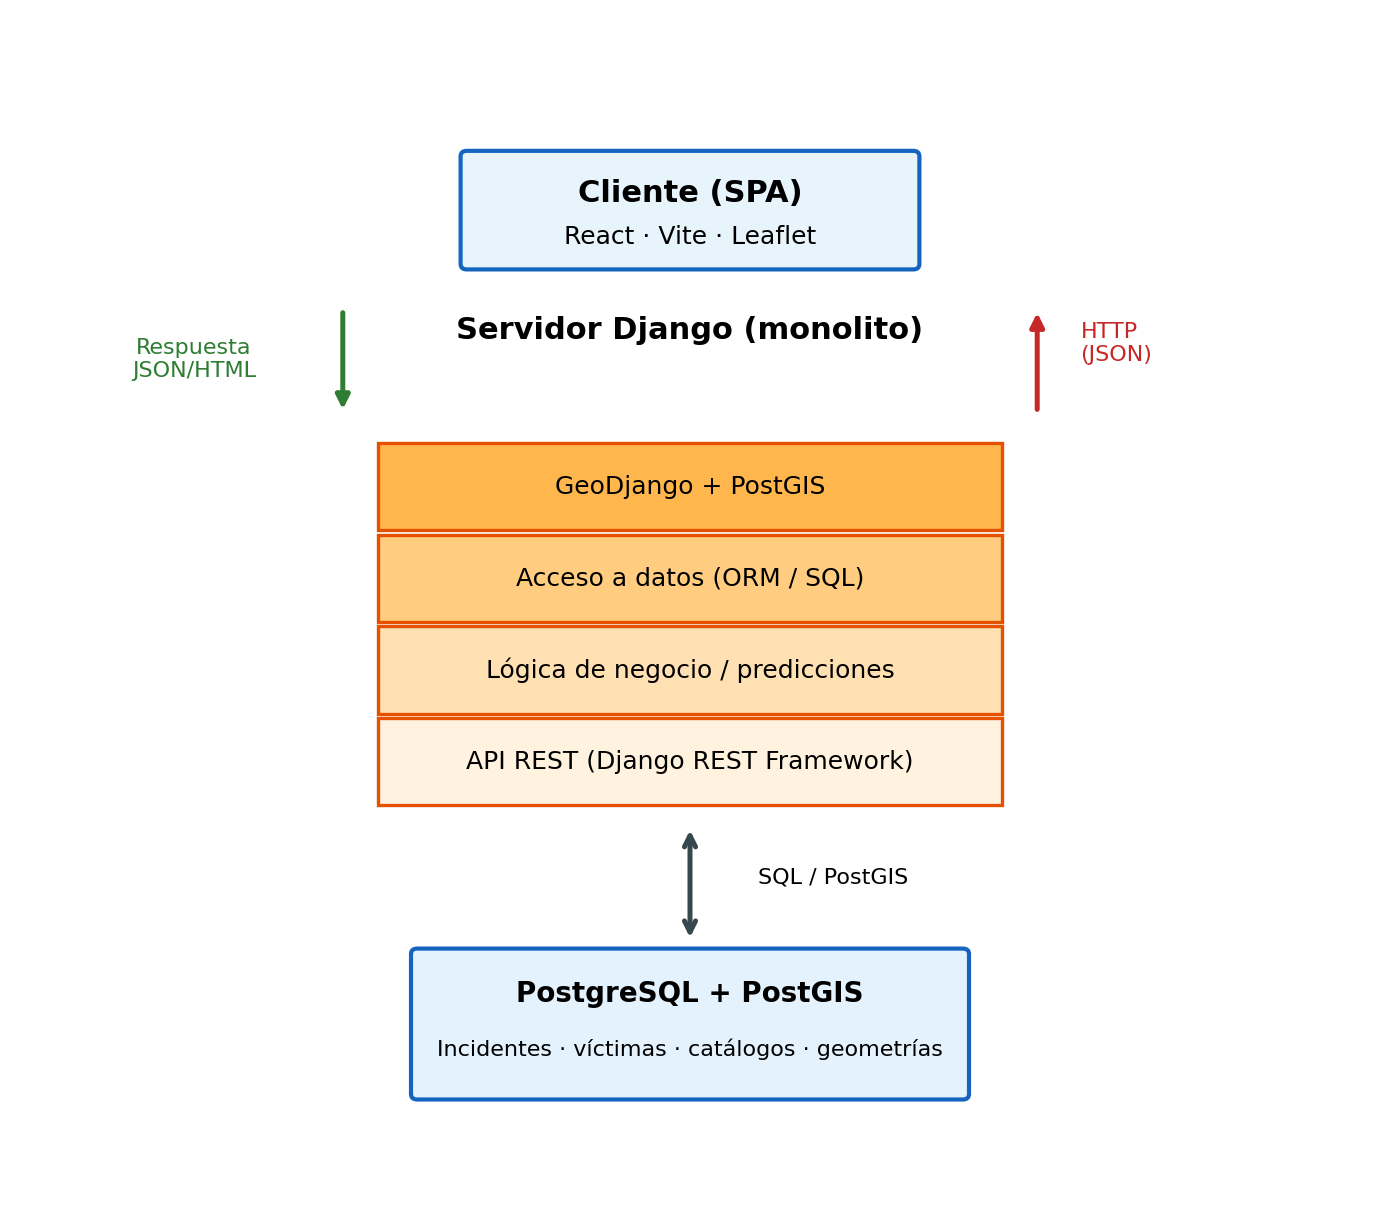
\includegraphics[width=0.75\linewidth]{images/fig_arquitectura_mtv.png}
	\caption{Patrón repositorio MTV en el backend de ViaData — Medellín}
	\label{fig:arquitectura-monolitica}
\end{figure}

\subsection{Sistemas de información geográficos y análisis espacial urbano}
Los \textbf{SIG} integran datos georreferenciados con atributos descriptivos (tipo de incidente, gravedad, franja horaria, entre otros), lo que permite estudiar \textbf{patrones territoriales y zonas críticas}. La literatura aplicada sostiene que los siniestros tienden a concentrarse en corredores e intersecciones asociados a infraestructura, flujo y comportamiento. Técnicas como la \textbf{estimación de densidad por núcleo} (KDE) y el \textbf{análisis de agrupación espacial} se emplean para identificar puntos calientes y priorizar intervenciones \cite{xu2022,li2023}.

\textbf{PostGIS} aporta tipos y operadores espaciales (\texttt{ST\_Contains}, índices espaciales); \textbf{GeoDjango} acerca esa capacidad al dominio de la aplicación. En el cliente, \textbf{Leaflet} y \textbf{react-leaflet} materializan capas de puntos, densidad y coroplética a partir de agregaciones del backend. ViaData — Medellín distingue además un \textbf{modo de territorio registro} ---filtro por comuna o barrio declarado en el registro Mede--- y un \textbf{modo espacial} ---asignación por polígono oficial a partir de coordenadas---, lo que permite contrastar la calidad cartográfica del dato mediante el indicador G03.

\begin{figure}[H]
	\centering
	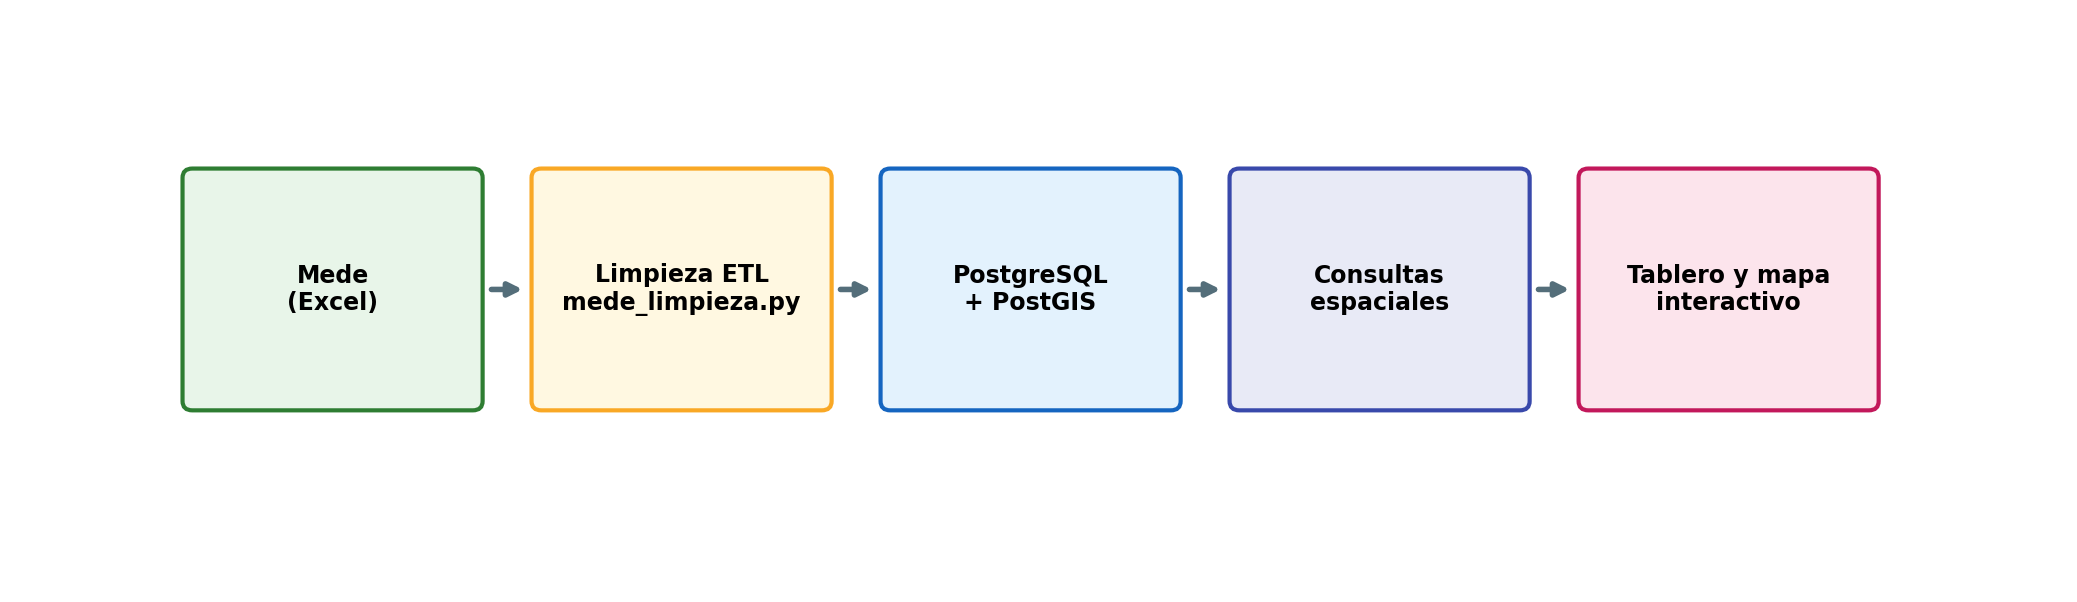
\includegraphics[width=0.95\linewidth]{images/fig_flujo_datos_geoespacial.png}
	\caption{Ciclo de vida de los datos geoespaciales (origen--destino)}
	\label{fig:flujo-de-datos-geoespacial}
\end{figure}

\subsection{Definiciones operativas en ViaData — Medellín}
Para evitar ambigüedades entre el lenguaje cotidiano de la seguridad vial y los cálculos del sistema, se adoptan las siguientes definiciones operativas:

\begin{table}[H]
	\centering
	\caption{Definiciones operativas del sistema}
	\label{tab:definiciones-operativas}
	\small
	\begin{tabularx}{\linewidth}{@{}l X@{}}
		\toprule
		\textbf{Término} & \textbf{Definición en ViaData — Medellín} \\
		\midrule
		Incidente & Evento de siniestro vial registrado en Mede; unidad de conteo distinta por identificador de incidente. \\
		Víctima & Persona asociada a un incidente; puede haber varias por evento. \\
		Víctima fatal & Clasificación según catálogo de gravedad (fatal, muerte, entre otras categorías equivalentes). \\
		Proyección & Escenario orientativo bajo estabilidad del patrón histórico filtrado; no implica causalidad. \\
		Hold-out & Validación que reserva los últimos meses del rango, entrena sin ellos y mide error al predecirlos. \\
		Participación por día & Porcentaje de incidentes en un día respecto al total del periodo; no es probabilidad individual. \\
		Modo registro / espacial & Filtro territorial por atributo declarado en Mede o por polígono PostGIS, respectivamente. \\
		\bottomrule
	\end{tabularx}
\end{table}

\clearpage

\subsection{Ciencia de datos, indicadores y tipos de modelos}
La ciencia de datos articula estadística, computación y dominio para convertir registros operativos en evidencia útil. En este proyecto el flujo incluye ingestión desde el Excel Mede, depuración centralizada, asociación a catálogos normalizados y carga a PostgreSQL/PostGIS; el análisis en tiempo de consulta combina SQL parametrizado y rutinas en NumPy. La solidez del análisis depende de la calidad del dato y de su integración con contexto territorial y temporal \cite{provost2022,atancuri2024}.

\subsubsection{Indicadores y analítica descriptiva / diagnóstica}
La medición de la siniestralidad se expresa en indicadores temporales, espaciales y de gravedad (frecuencia, severidad, tendencia). En el tablero y el mapa de ViaData — Medellín, KPIs, series mensuales, matrices día$\times$hora y rankings por comuna o barrio permiten la lectura diagnóstica del periodo seleccionado. El \textbf{índice de prioridad territorial P05} ---ponderación de frecuencia (30\,\%), densidad (15\,\%), tendencia (20\,\%), componente fatal (20\,\%) y participación relativa (15\,\%)--- materializa la lógica de priorización multicriterio sin recurrir a catálogos de vía o punto crítico, ausentes en la fuente Mede cargada \cite{parraga2024}.

\begin{figure}[H]
	\centering
	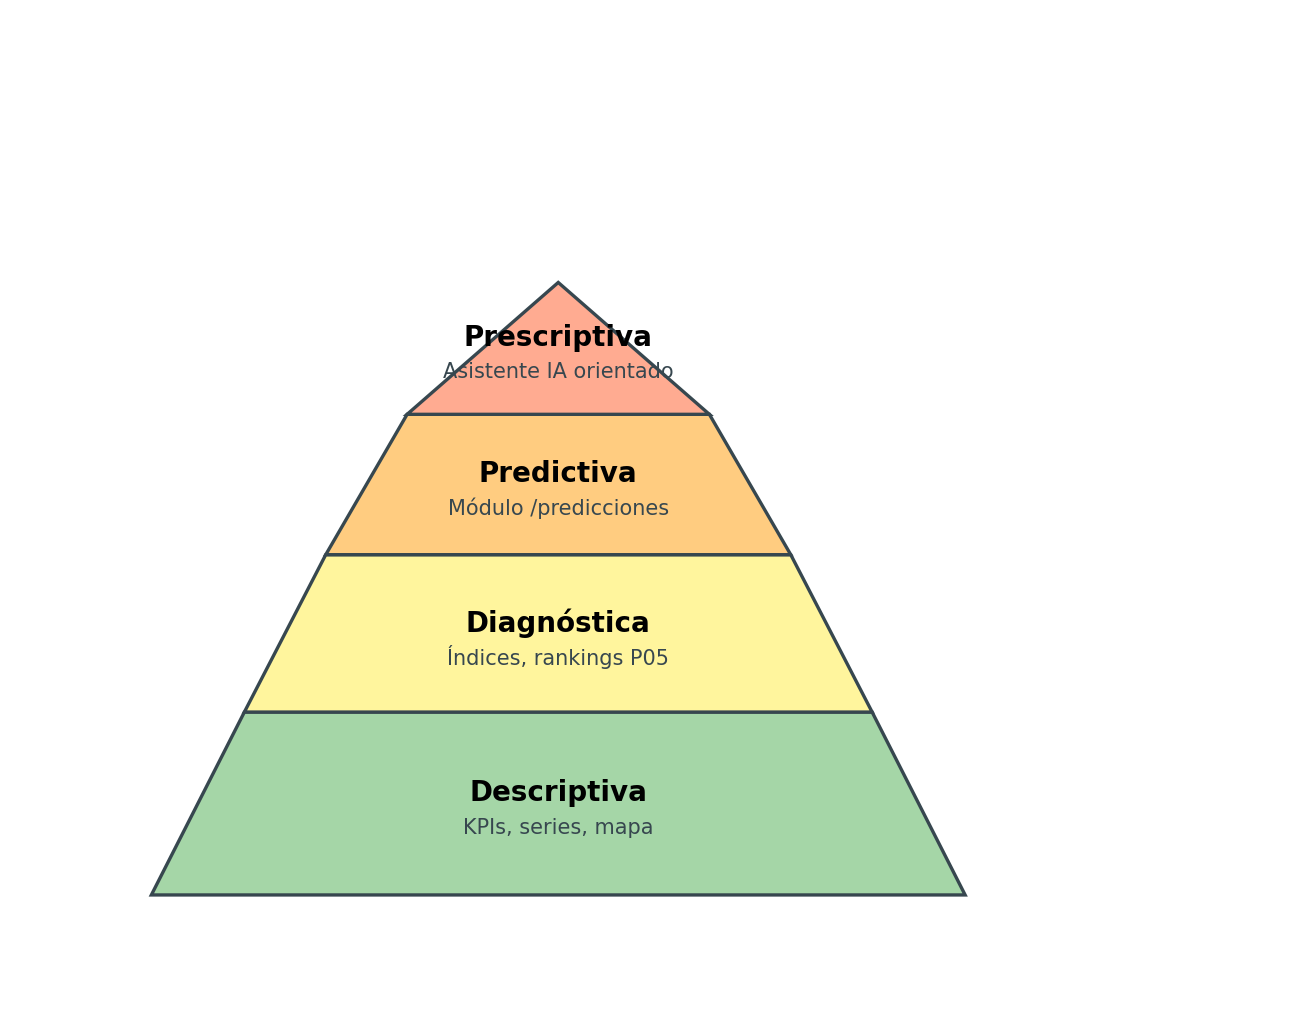
\includegraphics[width=0.8\linewidth]{images/fig_taxonomia_analitica.png}
	\caption{Taxonomía de analítica en ViaData — Medellín}
	\label{fig:arquitectura-monolitica-pagina-3}
\end{figure}

\subsubsection{Modelado de conteos y series temporales}
Los accidentes agregados por mes son variables de \textbf{conteo} con posible sobredispersión y estacionalidad intra-anual. En la literatura de accidentalidad se emplean, entre otros, modelos de \textbf{regresión de Poisson} o binomial negativa, \textbf{regresión lineal (OLS)} como línea base interpretable, y \textbf{ARIMA/SARIMA} cuando importa la memoria temporal y la estacionalidad mensual. ViaData — Medellín implementa variantes comparables en la interfaz ---OLS, diseño estacional, Poisson log-lineal, media móvil, bandas $\mu \pm 3\sigma$, ARIMA y SARIMA--- priorizando interpretabilidad y validación predictiva sobre modelos de caja negra \cite{lugo2025}.

Las series mensuales de Medellín combinan tendencia, estacionalidad y \textbf{shocks} estructurales ---como el confinamiento de mar–ago 2020---, por lo que el ajuste predictivo admite excluir esos meses del entrenamiento. Para proporciones ---porcentaje de víctimas fatales--- se requieren formulaciones distintas: regresión estacional sobre el porcentaje, \textbf{logit con exposición} o \textbf{ratio compuesto} al proyectar fatales y víctimas por separado.

\subsubsection{Validación predictiva: in-sample y hold-out}
El ajuste \textbf{in-sample} mide qué tan bien el modelo reproduce el periodo con el que fue estimado (R², MAPE in-sample), pero puede sobrevalorar modelos complejos. El esquema \textbf{hold-out} reserva los últimos $N$ meses del rango, entrena sin ellos y calcula el error al predecirlos; en ViaData — Medellín es el \textbf{criterio principal} para elegir modelo en proyección mensual y proporción de fatales. Se adopta como umbral exploratorio un MAPE hold-out $\leq 20\,\%$ (precisión estimada $\approx 100\,\% - \mathrm{MAPE}$), sin exigir R² $\geq 0{,}80$ en series mensuales perturbadas por la pandemia.

\begin{figure}[H]
	\centering
	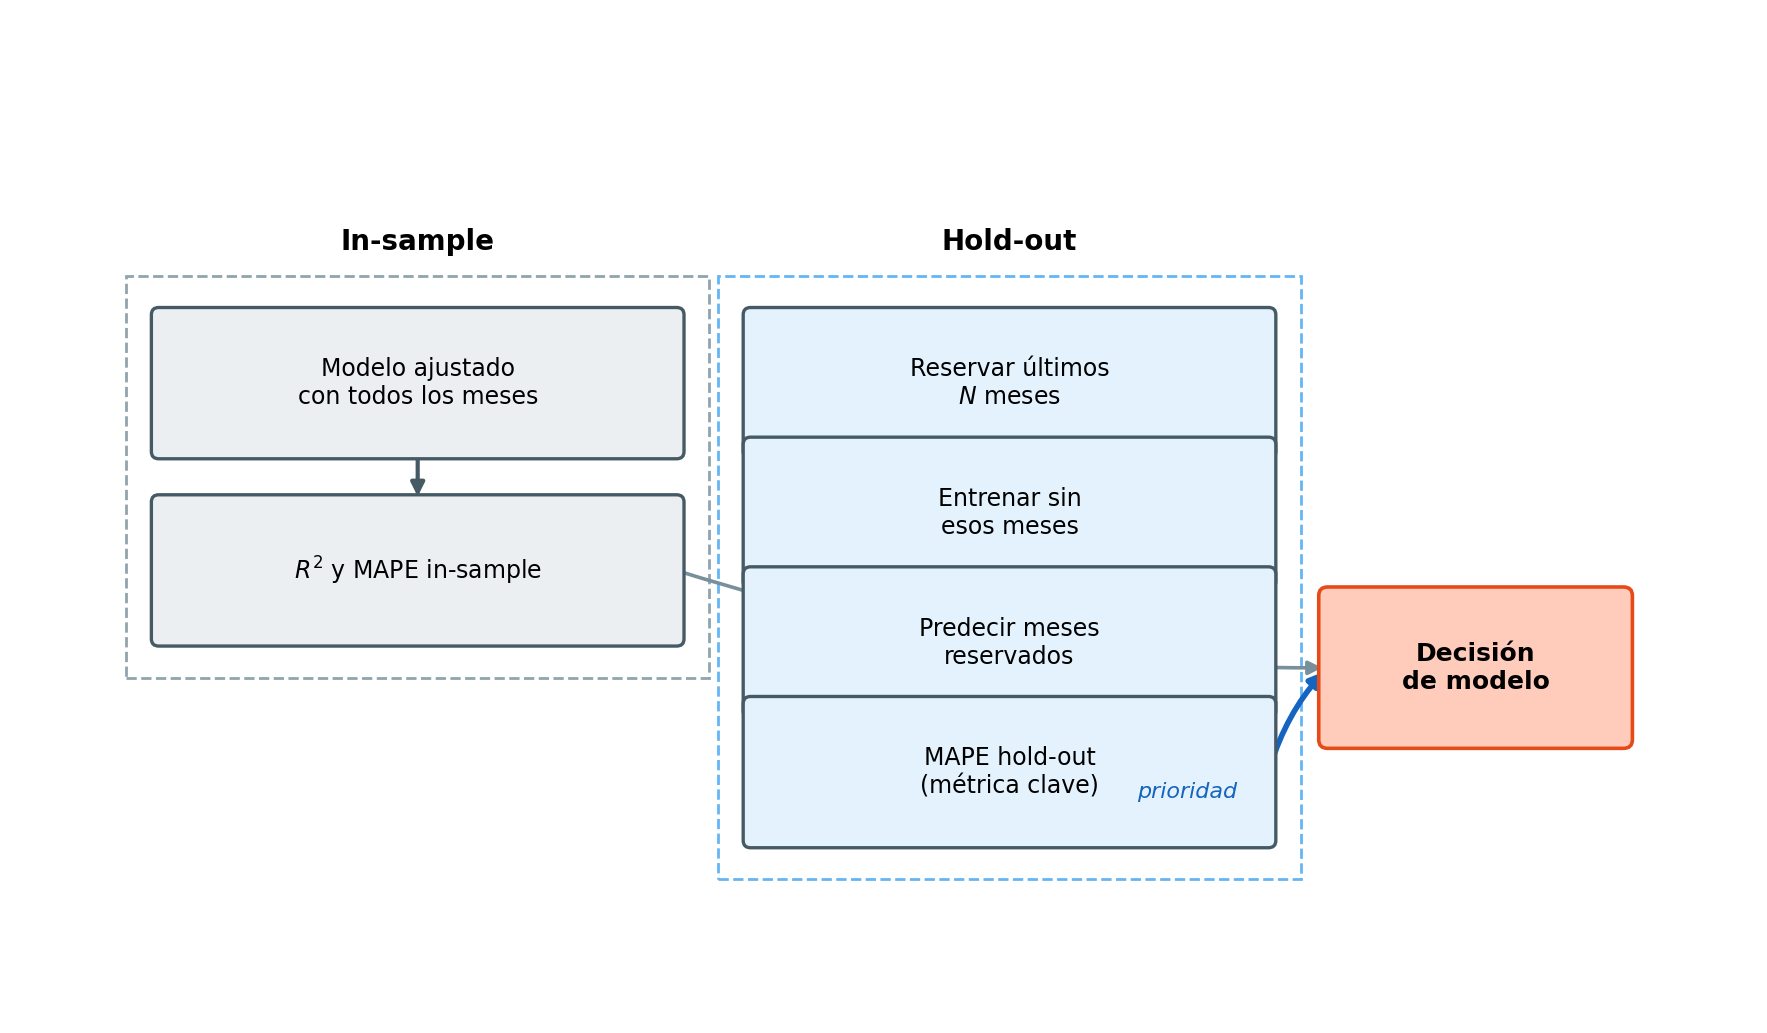
\includegraphics[width=0.90\linewidth]{images/fig_holdout_validacion.png}
	\caption{Esquema de validación in-sample frente a hold-out en el módulo de predicciones}
	\label{fig:holdout-validacion}
\end{figure}

\subsubsection{Familias de modelos en la plataforma}
\begin{itemize}[]
	\item \textbf{Formulaciones explícitas} (tasas, promedios, ponderaciones en SQL o servicios Django) actúan como modelos cerrados a escala de indicador, útiles en tablero y mapa.
	\item \textbf{Modelos empíricos y estadísticos} se apoyan en la historia operativa: agregaciones multidimensionales, comparación de periodos e índice P05, calculado como $0{,}30\,s_{\text{freq}} + 0{,}15\,s_{\text{dens}} + 0{,}20\,s_{\text{tend}} + 0{,}20\,s_{\text{fatal}} + 0{,}15\,s_{\text{part}}$ (cada $s$ en escala 0--100 dentro del territorio filtrado).
	\item \textbf{Modelos predictivos de series} se implementan con NumPy en rutinas propias (OLS, estacional, Poisson, media móvil, $\mu \pm 3\sigma$) y con \textbf{statsmodels} para ARIMA/SARIMA; no se emplean \texttt{scikit-learn} ni redes neuronales, por decisión de alcance orientada a transparencia y reproducibilidad.
\end{itemize}
Técnicas espaciales como KDE o cuadrículas de concentración (hotspots P14) complementan la lectura territorial cuando el volumen y la resolución del dato lo permiten \cite{xu2022,monar2025}.

\subsection{Taxonomía de indicadores del sistema}
Los indicadores de ViaData — Medellín se organizan en dos familias: \textbf{G} (geoespaciales y de calidad) y \textbf{P} (predictivos y de priorización). La Tabla~\ref{tab:taxonomia-indicadores} resume su propósito; el detalle de fórmulas y evaluación se presenta en metodología y resultados.

\begin{table}[H]
	\centering
	\caption{Taxonomía de indicadores G y P}
	\label{tab:taxonomia-indicadores}
	\small
	\begin{tabularx}{\linewidth}{@{}l l X@{}}
		\toprule
		\textbf{ID} & \textbf{Módulo} & \textbf{Pregunta analítica} \\
		\midrule
		G01--G02 & Mapa / tablero & Densidad de incidentes por km² \\
		G03 & Mapa / tablero & Coincidencia entre territorio registro y espacial \\
		G06 / P14 & Mapa & Concentración espacial (top celdas / hotspots) \\
		P01--P04 & Predicciones §1 & ¿Cuántos incidentes, víctimas o fatales por mes? \\
		P05 & Predicciones §2 & ¿Qué territorio priorizar en el periodo filtrado? \\
		P08--P10 & Predicciones §3 & ¿Qué territorio concentrará carga futura? \\
		P07 & Predicciones §4 & ¿Cómo evoluciona el \% de víctimas fatales? \\
		P12--P13 & Predicciones §5 & ¿Cuándo se concentrarían los incidentes (día y hora)? \\
		\bottomrule
	\end{tabularx}
\end{table}

\clearpage

\subsection{Roles, permisos y articulación del módulo predictivo}
El acceso a funcionalidades sigue un esquema de roles almacenado en perfil de usuario. Ciudadanos y visitantes sin autenticación consultan tablero, mapa y asistente con herramientas descriptivas; analistas y administradores acceden además a predicciones y reportes; solo el administrador gestiona cuentas. El rol autoridad se reserva para extensiones institucionales.

Los cinco bloques del módulo predictivo comparten filtros de fechas, territorio, clase de incidente y exclusión opcional de meses COVID, pero responden preguntas distintas. La proyección mensual (§1) alimenta el total de horizonte para patrones día$\times$hora (§5); la prioridad territorial (§2) mira el pasado reciente; la carga esperada (§3) orienta el ranking futuro por comuna o barrio; la proporción de fatales (§4) aporta el componente de gravedad relativa al índice P05. El diagrama de la Figura~\ref{fig:cadena-predictiva} resume esas dependencias conceptuales.

\begin{figure}[H]
	\centering
	\resizebox{\linewidth}{!}{%
	\begin{tikzpicture}[
		node distance=0.45cm and 0.5cm,
		mod/.style={draw, rounded corners, align=center, font=\scriptsize, inner sep=3pt, minimum width=2.4cm},
		filt/.style={draw, dashed, rounded corners, align=center, font=\scriptsize, inner sep=4pt, minimum width=5.8cm},
		arr/.style={-{Stealth[length=1.8mm]}, thick},
		darr/.style={-{Stealth[length=1.8mm]}, thick, dashed}
	]
		\node[filt] (f) {Filtros: fechas, territorio, clase, COVID};
		\node[mod, fill=blue!10, below left=1cm and 0.1cm of f] (s1) {§1 Proyección\\mensual};
		\node[mod, fill=green!12, below=1cm of f] (s2) {§2 Prioridad\\P05};
		\node[mod, fill=green!12, below right=1cm and 0.1cm of f] (s3) {§3 Carga\\territorial};
		\node[mod, fill=yellow!15, below left=1cm and 0.1cm of s1] (s4) {§4 \%\\fatales};
		\node[mod, fill=orange!12, below right=1cm and 0.1cm of s3] (s5) {§5 Patrones\\día$\times$hora};
		\draw[arr] (f) -- (s1); \draw[arr] (f) -- (s2);
		\draw[arr] (f) -- (s3); \draw[arr] (f) -- (s4); \draw[arr] (f) -- (s5);
		\draw[arr] (s1) -- node[above, font=\tiny, sloped] {total} (s5);
		\draw[darr] (s4) -- node[left, font=\tiny] {fatal} (s2);
		\draw[darr] (s2) -- node[below, font=\tiny] {ranking} (s3);
	\end{tikzpicture}%
	}
	\caption{Cadena conceptual de los bloques predictivos en ViaData — Medellín}
	\label{fig:cadena-predictiva}
\end{figure}

\subsubsection{Consulta en lenguaje natural}
El asistente conversacional incorpora un modelo de lenguaje (Google Gemini) con \textbf{function calling}: el sistema de diálogo selecciona herramientas que invocan las mismas rutas analíticas del backend, en lugar de generar SQL libre o cifras sin trazabilidad. Este enfoque separa la interacción en lenguaje natural del motor de cálculo y reduce el riesgo de respuestas numéricas inconsistentes \cite{carrillo2024}.

\clearpage

\subsection{Modelado de datos para analítica: estrella y copo de nieve}
En inteligencia de negocios y almacenes analíticos, \textbf{el modelo estrella} centraliza métricas en una tabla de hechos (p. ej., incidentes) y la rodea de dimensiones (tiempo, ubicación, tipo de evento). \textbf{El modelo copo de nieve} normaliza dimensiones en subdimensiones, reduciendo redundancia a cambio de consultas más complejas. La selección depende del equilibrio entre rendimiento, escalabilidad y mantenibilidad \cite{londono2024}.

En este trabajo el \textbf{esquema operacional} en PostgreSQL sigue un \textbf{modelo relacional normalizado} (catálogos, \texttt{incidente}, \texttt{victima}, vínculos geográficos), cercano al espíritu de un copo de nieve en las dimensiones de catálogo, mientras que las consultas tipo \textbf{OLAP} (conteos por fechas, comunas, clases) simulan hechos y dimensiones sin imponer un almacén separado. Si en el futuro se materializaran vistas analíticas dedicadas, el modelo estrella sería la referencia para exponer KPIs.

\begin{figure}[H]
	\centering
	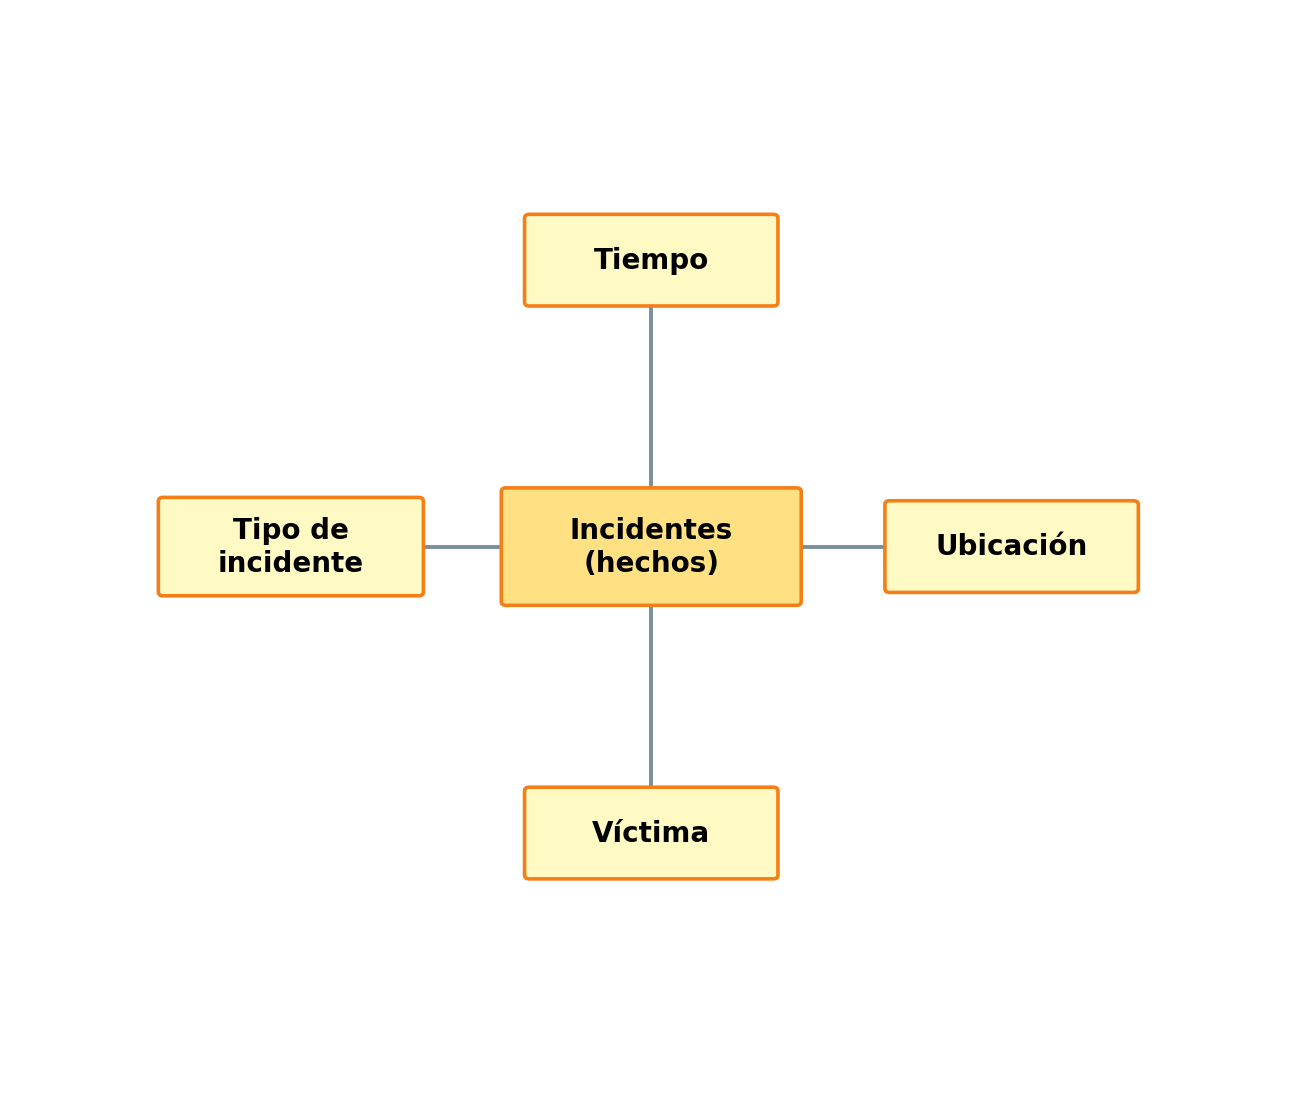
\includegraphics[width=0.65\linewidth]{images/fig_modelo_estrella.png}
	\caption{Modelo estrella (referencia conceptual)}
	\label{fig:arquitectura-monolitica-pagina-4}
\end{figure}

\begin{figure}[H]
	\centering
	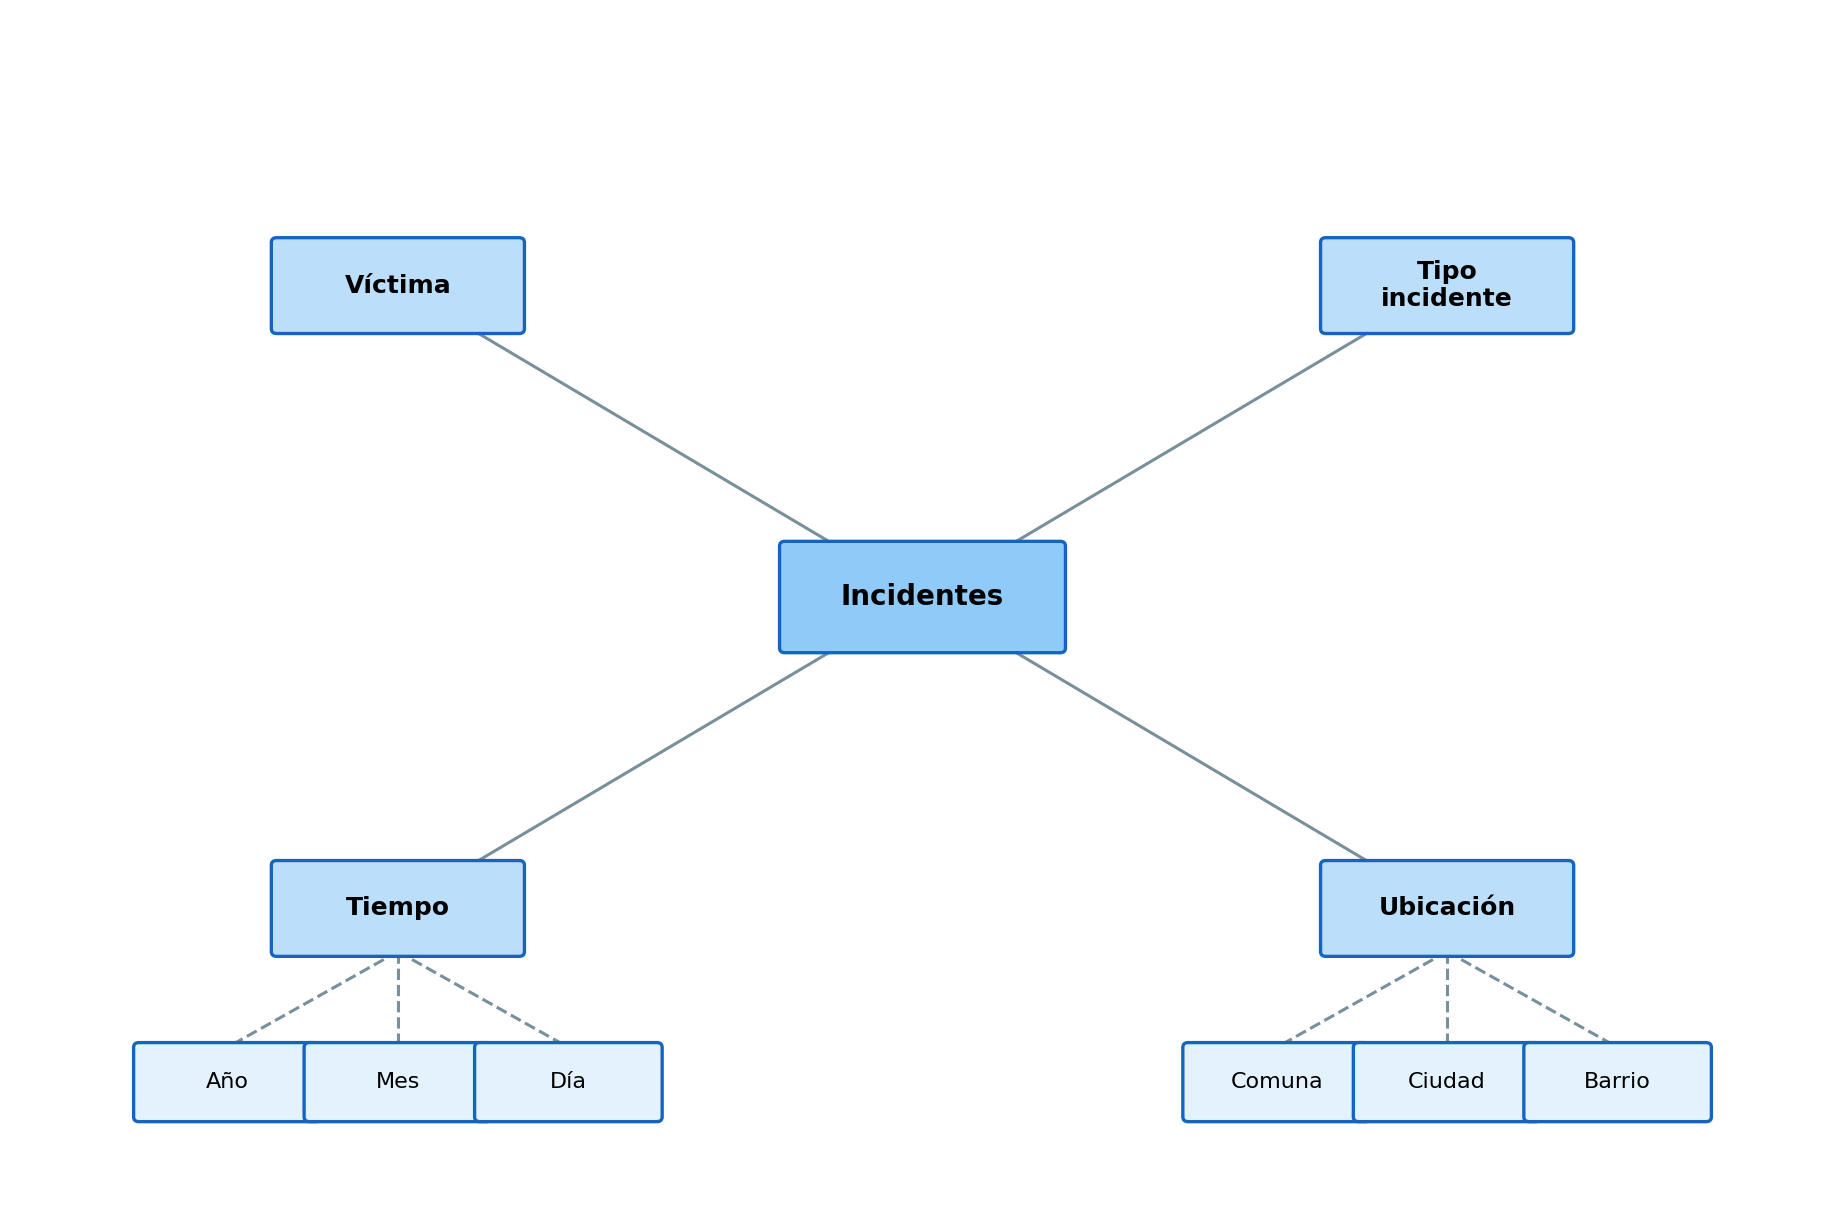
\includegraphics[width=0.85\linewidth]{images/fig_modelo_copo_nieve.png}
	\caption{Modelo copo de nieve aplicado a incidentes y dimensiones}
	\label{fig:arquitectura-monolitica-pagina-6}
\end{figure}

\subsection{Visualización analítica, tableros y experiencia de usuario}
Los dashboards integran gráficos, mapas y tablas dinámicas bajo filtros compartidos (fechas, territorio, clase, gravedad). La analítica visual apoya la decisión en entornos urbanos con información abundante y heterogénea \cite{monar2025}. En ViaData — Medellín, \textbf{mapas de calor, rankings territoriales, hotspots y series temporales} permiten detectar patrones y focalizar intervenciones. Los contratos de \textbf{API} conservan la misma semántica de indicadores en tablero, mapa, predicciones y asistente, de modo que un mismo filtro territorial produce resultados comparables entre módulos.

\subsection{Calidad y gobernanza de los datos}
La efectividad de la plataforma depende de la calidad del dato: estandarización, consistencia, trazabilidad desde Mede hasta el indicador expuesto y documentación de reglas de depuración en un único módulo ETL. Sin indicadores estructurados y gobernanza, los sistemas analíticos difícilmente sostienen políticas de seguridad vial basadas en evidencia \cite{oviedo2025,oms2024}. En ViaData — Medellín, la gobernanza se traduce en validación y normalización a catálogos, integridad referencial en la base, contraste registro--espacial (G03) y procesos de carga reproducibles, de modo que la plataforma funcione como infraestructura de conocimiento y no solo como reportes aislados.


\section{METODOLOGÍA}
\subsection{Enfoque general de la investigación}

La presente investigación adopta un enfoque metodológico de tipo \textbf{aplicado} con orientación \textbf{cuantitativa}, centrado en el diseño, la implementación y la evaluación de \textbf{ViaData — Medellín}: un instrumento virtual geoespacial para organizar, visualizar y proyectar la accidentalidad vial en Medellín a partir de datos históricos oficiales. El estudio articula de manera secuencial ingeniería de software, ciencia de datos y sistemas de información geográfica, de modo que los registros administrativos Mede se transformen en indicadores, mapas y escenarios orientativos con trazabilidad en los cálculos \cite{changotasig2023,lugo2025}.

A diferencia de un análisis puramente descriptivo, la metodología incorpora \textbf{analítica predictiva} con modelos estadísticos transparentes (OLS, estacional, Poisson, media móvil, bandas $\mu \pm 3\sigma$, ARIMA y SARIMA) y validación \textit{hold-out}, además de índices de priorización y carga territorial. Las proyecciones se interpretan como escenarios bajo estabilidad del patrón histórico filtrado: apoyan la planificación y la lectura comparativa, pero \textbf{no establecen causalidad} ni probabilidad individual de sufrir un siniestro \cite{oms2024,parraga2024}. La Figura~\ref{fig:diagrama-de-metodologia} resume las fases del proceso.

\begin{figure}[H]
	\centering
	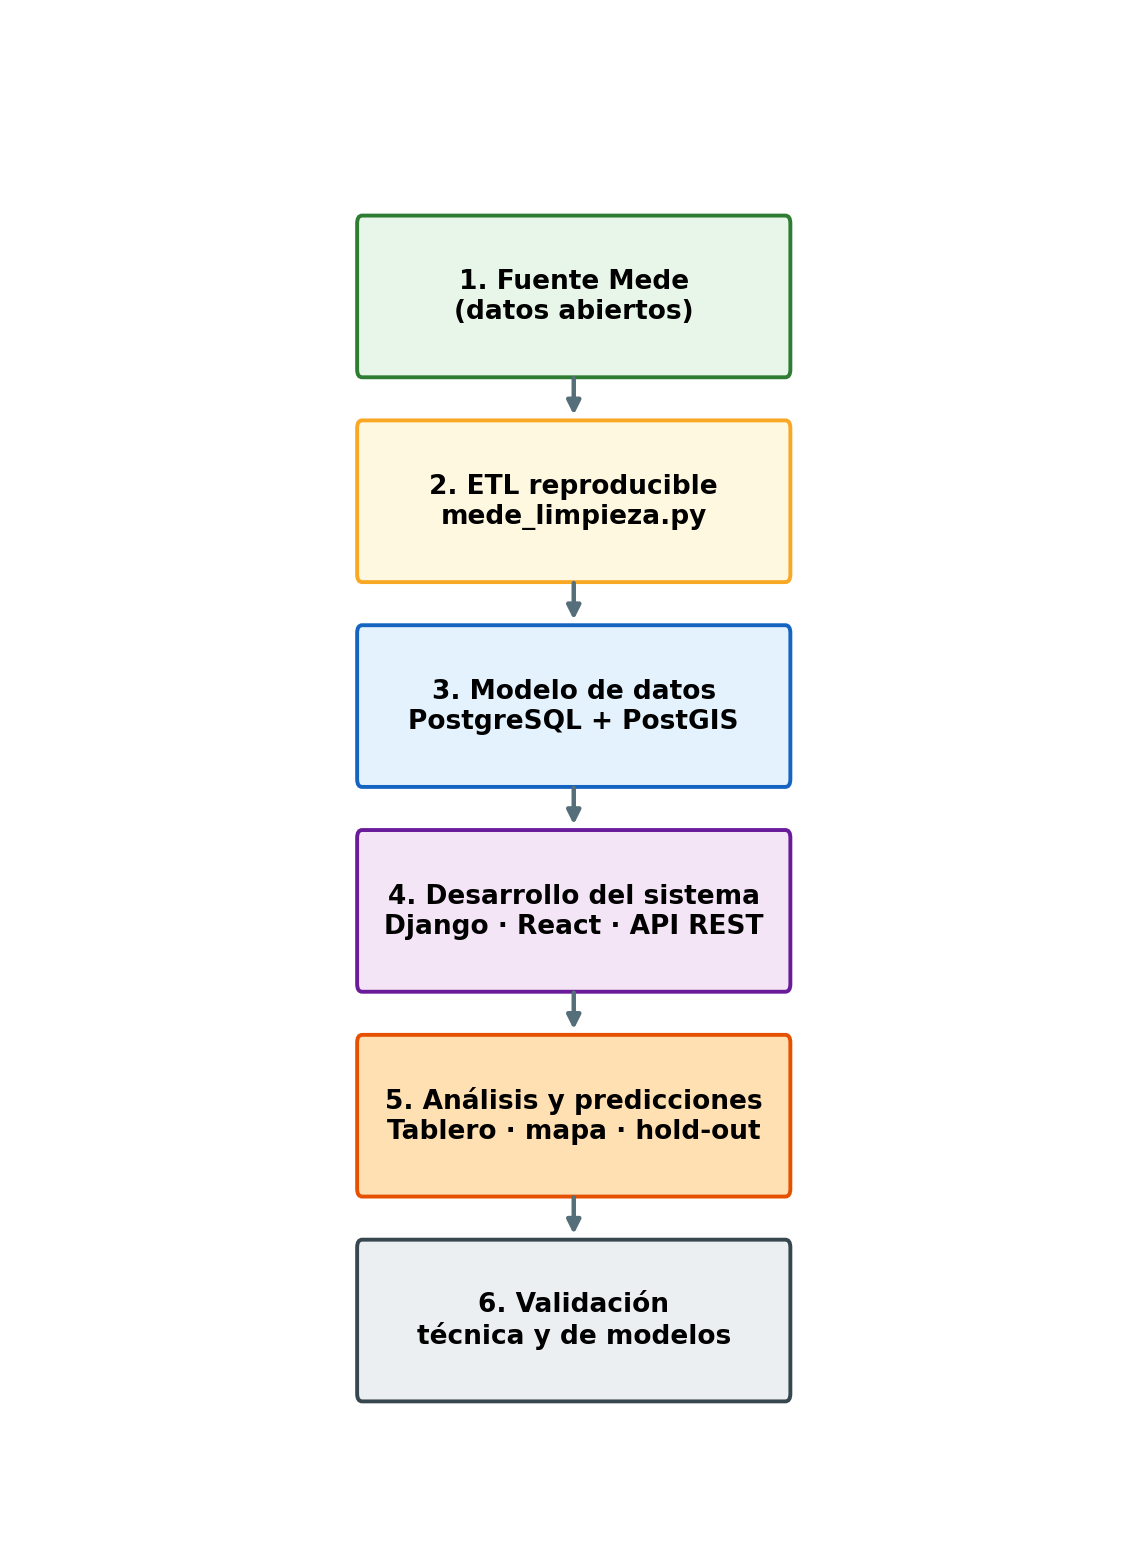
\includegraphics[width=0.62\linewidth]{images/fig_metodologia.png}
	\caption{Fases metodológicas de ViaData — Medellín}
	\label{fig:diagrama-de-metodologia}
\end{figure}

\subsection{Fuentes de datos y proceso ETL}

La fuente principal corresponde al conjunto de datos abiertos \textbf{Mede} publicado en la plataforma institucional de Medellín (\texttt{Mede\_Victimas\_inci.xlsx}), que concentra registros de incidentes y víctimas con variables temporales, territoriales, de gravedad y georreferenciación. El periodo típico cargado en la base del proyecto abarca aproximadamente \textbf{2014-01-01 — 2021-09-30}, con del orden de \textbf{160\,000+} incidentes con coordenadas válidas tras depuración, según el Excel y los indicadores de calidad del pipeline \cite{atancuri2024}.

La ingestión sigue un flujo \textbf{ETL reproducible} documentado y versionado. En primer lugar, el módulo \texttt{mede\_limpieza.py} concentra las reglas únicas de depuración (\texttt{depurar\_mede}), evitando duplicar lógica en otros scripts. A partir del Excel se genera \texttt{Mede\_Victimas\_inci\_depurado.csv}; el script \texttt{carga\_mede\_pgadmin.sql} realiza la carga idempotente a PostgreSQL; y los scripts PostGIS (\texttt{001}–\texttt{006}) más la carga de polígonos oficiales habilitan la asignación territorial espacial. Scripts auxiliares (\texttt{mede\_eda\_export.py}, \texttt{mede\_pipeline\_guiado.py}) apoyan el análisis exploratorio y la verificación de checkpoints. Este diseño garantiza que la memoria de grado, el EDA y la aplicación web describan el \textbf{mismo comportamiento} de limpieza \cite{provost2022}.

\begin{figure}[H]
	\centering
	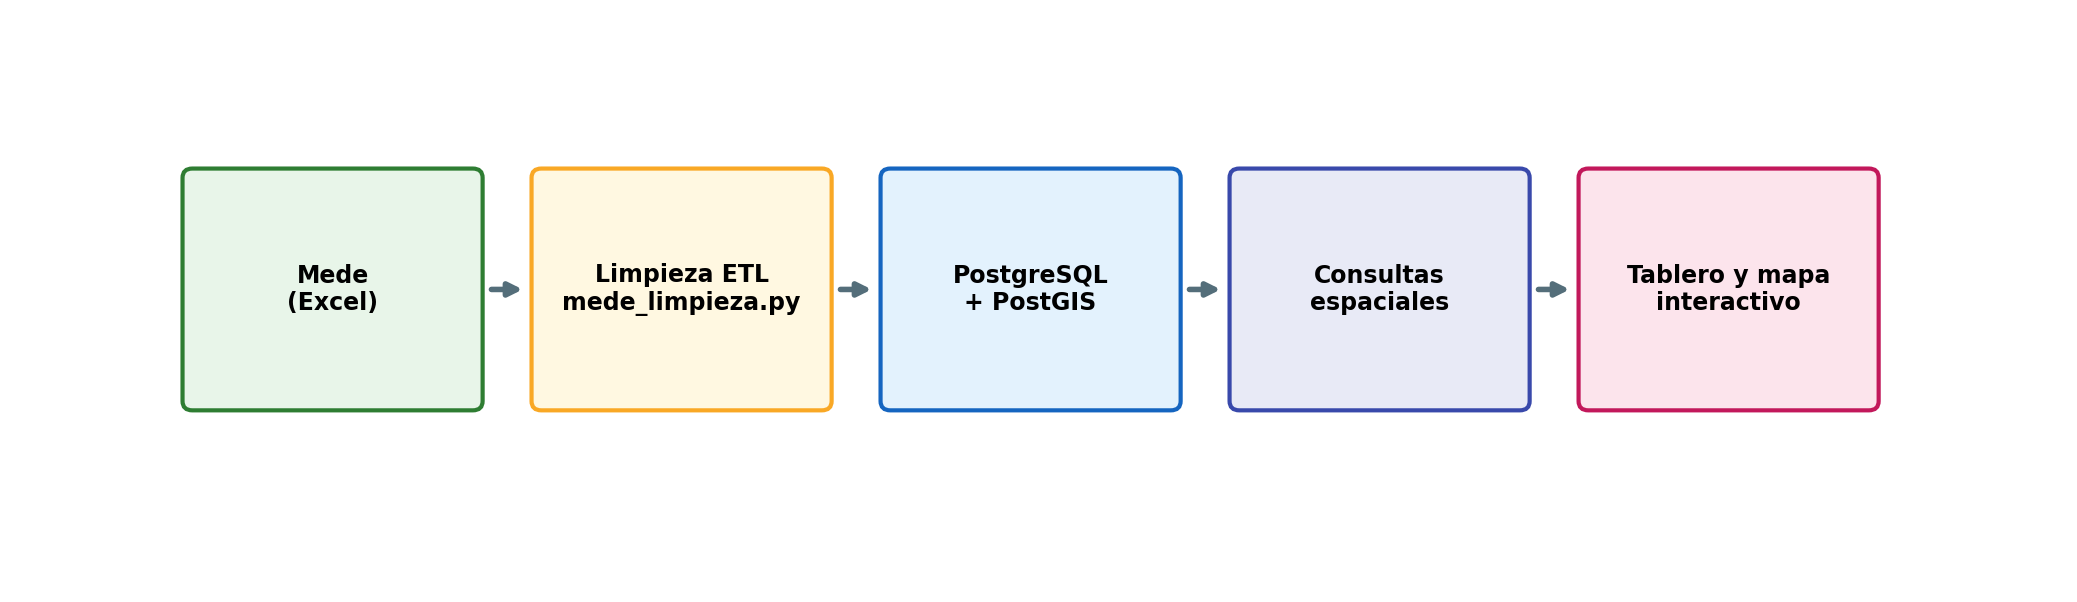
\includegraphics[width=0.95\linewidth]{images/fig_flujo_datos_geoespacial.png}
	\caption{Flujo de datos desde Mede hasta la visualización geoespacial}
	\label{fig:metodologia-flujo-etl}
\end{figure}

En la etapa de depuración se abordan inconsistencias de formato, valores faltantes, normalización de catálogos (tipo de incidente, clase, gravedad) y validación de coordenadas. La calidad del análisis posterior depende directamente de esta fase; el indicador G03 del sistema permite contrastar, una vez cargados los polígonos, la coincidencia entre el territorio declarado en el registro y el asignado espacialmente.

\subsection{Diseño del modelo de datos y territorio espacial}

El modelo relacional estructura la información en entidades normalizadas ---incidentes, víctimas y catálogos asociados--- con geometrías gestionadas por PostGIS. Cada incidente conserva atributos descriptivos y un punto geográfico cuando las coordenadas son válidas. ViaData — Medellín distingue dos modos de lectura territorial: \textbf{modo registro} (filtro por comuna o barrio declarado en Mede) y \textbf{modo espacial} (asignación por polígono oficial a partir de coordenadas), lo que permite evaluar la calidad cartográfica del dato y sostener agregaciones comparables en tablero, mapa y predicciones.

\subsection{Arquitectura e implementación del sistema}

El desarrollo adopta una \textbf{arquitectura monolítica} en Django que concentra autenticación JWT, API REST (Django REST Framework), lógica analítica y acceso a datos, mientras el frontend React (Vite) opera como aplicación de página única. Las apps \texttt{accounts}, \texttt{dashboard}, \texttt{agent} y \texttt{reports} cubren, respectivamente, usuarios y roles, KPIs y predicciones, asistente conversacional con herramientas sobre la API, y payloads para reportes imprimibles. GeoDjango y PostgreSQL/PostGIS soportan consultas espaciales; Leaflet y \texttt{react-leaflet} materializan capas en el cliente. Los cálculos predictivos emplean NumPy en rutinas propias y \textbf{statsmodels} para ARIMA/SARIMA; el ETL offline usa pandas según \texttt{requirements-etl.txt}. La Figura~\ref{fig:arquitectura-monolitica} del marco conceptual detalla el patrón MTV del backend.

\subsection{Procesamiento analítico y módulo de predicciones}

El procesamiento combina consultas SQL parametrizadas en tiempo de petición con rutinas numéricas en el backend. En el plano \textbf{descriptivo y diagnóstico}, el tablero y el mapa calculan KPIs, series mensuales, distribuciones por día y hora, densidades territoriales (G01--G02), rankings por comuna o barrio y concentraciones espaciales (G06/P14) mediante KDE o cuadrículas cuando el volumen lo permite \cite{xu2022,monar2025}.

El módulo de \textbf{predicciones} organiza cinco bloques analíticos con filtros compartidos (fechas, territorio, clase de incidente, exclusión opcional de mar–ago 2020):

\begin{itemize}
	\item \textbf{§1 Proyección mensual} (P01--P04): compara siete familias de modelos sobre conteos mensuales de incidentes, víctimas o fatales.
	\item \textbf{§2 Prioridad territorial} (P05): índice multicriterio fijo sobre el periodo filtrado, sin entrenamiento predictivo.
	\item \textbf{§3 Carga territorial} (P08--P10): proyección de volumen futuro por comuna o barrio.
	\item \textbf{§4 Proporción de fatales} (P07): modelos sobre el porcentaje de víctimas fatales.
	\item \textbf{§5 Patrones temporales} (P12--P13): reparto día$\times$hora a partir del total proyectado en §1.
\end{itemize}

La cadena de dependencias entre bloques se presenta en la Figura~\ref{fig:cadena-predictiva} del marco conceptual. El alcance deliberadamente \textbf{no incluye} ranking automatizado por vía o punto crítico ---ausente en Mede--- ni modelos de aprendizaje automático espacial avanzado; la ingesta de datos nuevos permanece como proceso manual reproducible.

\subsection{Protocolo de evaluación de modelos}

La evaluación predictiva distingue ajuste \textbf{in-sample} y validación \textbf{hold-out}: se reservan los últimos $N$ meses del rango, se entrena sin ellos y se mide el error al predecirlos. El hold-out es el \textbf{criterio principal} para seleccionar modelo en §1 y §4; se adopta como umbral exploratorio un MAPE hold-out $\leq 20\,\%$ (precisión estimada $\approx 100\,\% - \mathrm{MAPE}$), sin exigir R$^2 \geq 0{,}80$ en series mensuales perturbadas por la pandemia. La Figura~\ref{fig:holdout-validacion} del marco conceptual ilustra este esquema.

La Tabla~\ref{tab:config-evaluacion} resume la configuración estándar del escenario de referencia A; la Tabla~\ref{tab:protocolo-bloques} especifica la métrica y la decisión adoptada por bloque. Los scripts \texttt{llenar\_evaluacion\_seccion*.py} y los CSV en \texttt{evaluaciones/} aseguran reproducibilidad numérica; los resultados detallados se reportan en la sección de resultados.

\begin{table}[h]
	\centering
	\caption{Configuración estándar de evaluación predictiva (escenario A)}
	\label{tab:config-evaluacion}
	\small
	\begin{tabularx}{\linewidth}{@{}l X@{}}
		\toprule
		\textbf{Parámetro} & \textbf{Valor} \\
		\midrule
		Periodo de referencia & 2018-01-01 — 2021-09-30 \\
		Excluir mar–ago 2020 del ajuste & Sí (opción por defecto en la interfaz) \\
		Hold-out & 3 meses (6 opcionales en §1 y §4) \\
		Horizonte de proyección & 3 meses \\
		Escenarios §1 & A–I (ciudad, variable, territorio, clase, COVID, rangos cortos) \\
		\bottomrule
	\end{tabularx}
\end{table}

\begin{table}[h]
	\centering
	\caption{Protocolo de evaluación por bloque del módulo de predicciones}
	\label{tab:protocolo-bloques}
	\small
	\begin{tabularx}{\linewidth}{@{}l c X l@{}}
		\toprule
		\textbf{Bloque} & \textbf{¿Modelos?} & \textbf{Métrica principal} & \textbf{Decisión} \\
		\midrule
		§1 Proyección mensual & Sí (7 $\times$ 9 escenarios) & MAPE hold-out & SARIMA ciudad incidentes \\
		§2 Prioridad territorial & No (índice fijo) & Spearman índice$\leftrightarrow$frecuencia & P05 comunas referencia \\
		§3 Carga territorial & Sí (6 en A; estacional en B–G) & Spearman carga$\leftrightarrow$volumen & Estacional territorial \\
		§4 Proporción fatales & Sí (8 en A) & MAPE hold-out sobre \% & Estacional sobre \% \\
		§5 Patrones temporales & Hereda §1 & Spearman patrón obs.$\leftrightarrow$proy. & Patrón estable; hereda §1 \\
		\bottomrule
	\end{tabularx}
\end{table}

Para la proyección mensual de incidentes a nivel ciudad, el modelo adoptado tras la evaluación es \textbf{SARIMA$(2,1,3)(1,1,1)_{12}$} implementado con statsmodels, con media móvil de tres meses como alternativa interpretable. El índice P05 se valida por correlación de Spearman con la frecuencia observada en comunas de referencia; la carga territorial y los patrones día$\times$hora se evalúan por coherencia de ranking y estabilidad del patrón, respectivamente.

\subsection{Validación técnica del software}

Complementariamente a la evaluación de modelos, la metodología contempla \textbf{validación técnica del sistema}: pruebas automatizadas con \texttt{pytest} y \texttt{pytest-django} sobre las apps \texttt{dashboard}, \texttt{agent}, \texttt{accounts} y \texttt{reports}; verificación de endpoints críticos de la API; y revisión de desempeño en consultas frecuentes a PostgreSQL/PostGIS. Esta fase responde al objetivo específico de validar desempeño, seguridad y escalabilidad de la plataforma, y se complementa con la coherencia de indicadores y la utilidad de tablero, mapa y reportes para el análisis de accidentalidad.

En conjunto, el proceso metodológico integra desarrollo tecnológico, calidad del dato, analítica descriptiva/diagnóstica/predictiva y validación reproducible, transformando datos abiertos Mede en un instrumento geoespacial consultable que responde a los objetivos planteados y deja trazabilidad para extensiones futuras documentadas en trabajo futuro.

\subsection{Instrumentos y técnicas de recolección y análisis de datos}

La investigación se fundamenta en \textbf{fuentes secundarias} estructuradas: el dataset Mede como instrumento principal de recolección indirecta. No se aplican encuestas ni instrumentos de campo; la evidencia empírica proviene de registros administrativos ya consolidados por la institución.

Para el procesamiento se emplean Python (\texttt{pandas}, \texttt{numpy}) en el ETL offline; SQL y GeoDjango/PostGIS en consultas y agregaciones; NumPy y statsmodels en modelos de series; y bibliotecas de visualización en el cliente (Recharts, Leaflet). Las técnicas de análisis abarcan analítica descriptiva y diagnóstica (KPIs, distribuciones, índice P05), análisis geoespacial (densidad, coroplética, asignación territorial), modelado de conteos y series temporales con validación hold-out, y generación de reportes exportables. La reproducibilidad del ETL y de las evaluaciones numéricas constituye un criterio transversal del diseño metodológico.

\subsection{Población y muestra}

La \textbf{población} objeto de estudio está conformada por el conjunto total de registros de accidentes de tránsito ocurridos en Medellín y reportados en Mede dentro del periodo disponible en el dataset cargado. Incluye distintos tipos de incidente, actores viales, condiciones y niveles de gravedad según la estructura del archivo fuente.

Dado que el estudio se basa en datos secundarios, no se realiza muestreo probabilístico en sentido tradicional: se trabaja con la \textbf{totalidad de los registros} disponibles tras depuración (enfoque censal), lo que reduce sesgos de selección y permite analizar el fenómeno de manera integral \cite{oviedo2025}. Para fines analíticos, la plataforma aplica filtros temporales, geográficos y categóricos que segmentan la población en subconjuntos ---periodos, comunas, clases de incidente, rangos con o sin exclusión COVID--- sin constituir muestras independientes, sino estrategias de exploración y evaluación bajo escenarios documentados.


\section{RESULTADOS}
\subsection{Entrega del sistema ViaData — Medellín}

El desarrollo culminó en una plataforma web funcional que integra backend Django con API REST, base PostgreSQL/PostGIS y frontend React. Los módulos entregados cubren mapa analítico (\texttt{/}, \texttt{/mapa}), tablero de indicadores (\texttt{/tablero}), predicciones (\texttt{/predicciones}), reportes imprimibles (\texttt{/reporte/vista}), asistente conversacional (\texttt{/agente}) y gestión de usuarios (\texttt{/admin/usuarios}), con autenticación JWT y roles diferenciados (ciudadano, analista, administrador). El módulo de predicciones fue evaluado y cerrado el 18 de junio de 2026 con evidencia reproducible en archivos CSV y scripts de evaluación.

\subsection{Cumplimiento de objetivos}

La Tabla~\ref{tab:cumplimiento-objetivos} relaciona los objetivos planteados con la evidencia observable en el sistema. Los componentes complementarios (mapa, reportes, asistente y administración de usuarios) se reportan como entregables de apoyo, sin ampliar la formulación original de objetivos.

\begin{table}[H]
	\centering
	\caption{Cumplimiento de objetivos y componentes de ViaData — Medellín}
	\label{tab:cumplimiento-objetivos}
	\small
	\begin{tabularx}{\linewidth}{@{}l X c@{}}
		\toprule
		\textbf{Elemento} & \textbf{Evidencia en el sistema} & \textbf{Estado} \\
		\midrule
		Objetivo general & Instrumento geoespacial con visualización, análisis, segmentación y modelos estadísticos orientativos & Cumplido \\
		OE1: arquitectura y modelo de datos & Monolito Django + PostGIS; ETL \texttt{mede\_limpieza.py}; entidades incidente/víctima/catálogos & Cumplido \\
		OE2: módulos de análisis estadístico & KPIs, rankings, índice P05, proyecciones §1--§5, densidad y hotspots & Cumplido \\
		OE3: tablero de monitoreo & Series mensuales, matrices día$\times$hora, filtros territoriales y temporales & Cumplido \\
		OE4: validación técnica & Suite \texttt{pytest} en apps críticas; consultas PostGIS verificables & Cumplido \\
		Mapa analítico (complementario) & Puntos, heatmap, coroplética, G03, modo registro/espacial & Entregado \\
		Reportes y asistente (complementarios) & Exportación imprimible; Gemini con herramientas sobre la API & Entregado \\
		\bottomrule
	\end{tabularx}
\end{table}

\subsection{Carga de datos y calidad de la base}

Tras el pipeline ETL documentado, la base operativa concentra registros Mede entre \textbf{2014-01-01} y \textbf{2021-09-30}, con del orden de \textbf{160\,000+} incidentes con coordenadas válidas. En el escenario de referencia A (2018--2021, exclusión COVID en el ajuste), el periodo filtrado para priorización territorial registra \textbf{75\,088} incidentes a nivel ciudad y \textbf{22} comunas elegibles.

El indicador \textbf{G03} cuantifica la coincidencia entre el territorio declarado en el registro Mede y el asignado espacialmente por polígono oficial. En modo espacial PostGIS, el escenario A de prioridad territorial reporta \textbf{66\,137} incidentes con \textbf{21} comunas elegibles, lo que permite contrastar la lectura administrativa frente a la cartográfica. La depuración centralizada en \texttt{mede\_limpieza.py} asegura coherencia entre el análisis exploratorio, la carga a PostgreSQL y los cálculos expuestos en la interfaz.

\subsection{Resultados descriptivos y geoespaciales}

El tablero y el mapa materializan la analítica descriptiva y diagnóstica sobre el periodo y los filtros seleccionados por el usuario. La Figura~\ref{fig:captura-tablero} muestra los KPIs del escenario de referencia (ciudad completa, 2018--2021): \textbf{75\,088} incidentes ($-2{,}69\,\%$ frente al año anterior), \textbf{108\,541} víctimas y \textbf{703} fatales ($+1{,}01\,\%$). Entre los hallazgos recurrentes destacan:

\begin{itemize}
	\item \textbf{Concentración territorial:} La Candelaria encabeza rankings por volumen en múltiples cortes (75\,088 incidentes ciudad; 12\,921 en La Candelaria en escenario A de prioridad).
	\item \textbf{Patrón temporal:} La celda líder día$\times$hora histórica es \textbf{martes 07:00}; el día con mayor participación relativa es \textbf{martes} (patrones P12/P13, escenario A).
	\item \textbf{Gravedad relativa:} El porcentaje mensual observado de víctimas fatales en ciudad se sitúa en torno a \textbf{0,66\,\%} (rango 0,35--1,2\,\%), con variabilidad mensual elevada.
	\item \textbf{Calidad espacial:} El modo registro frente al modo espacial produce rankings comparables en comunas (Spearman índice$\leftrightarrow$frecuencia $\approx 0{,}86$ en modo espacial), útil para discutir la confiabilidad cartográfica del dato \cite{monar2025}.
\end{itemize}

\begin{figure}[H]
	\centering
	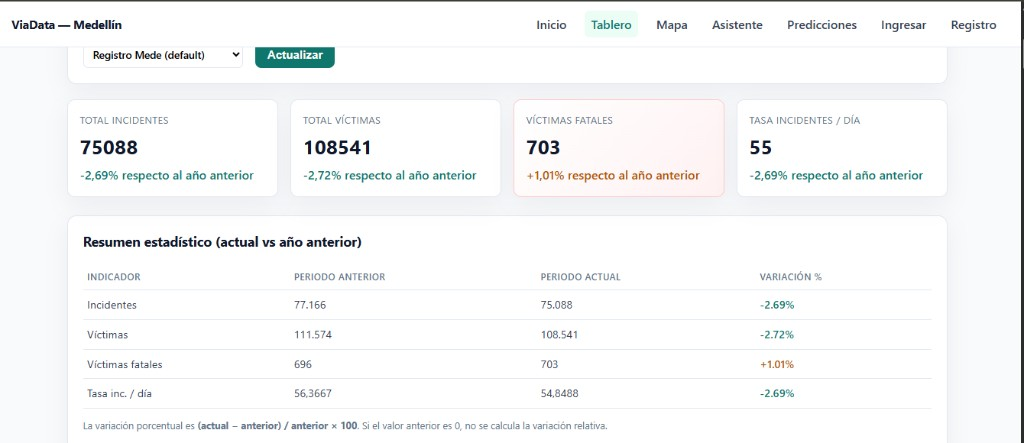
\includegraphics[width=0.92\linewidth]{images/captura_tablero.png}
	\caption{Tablero de indicadores — KPIs y resumen estadístico (ciudad completa, 2018--2021)}
	\label{fig:captura-tablero}
\end{figure}

La Figura~\ref{fig:captura-mapa-densidad} ilustra la capa de \textbf{densidad territorial} (G01--G02) en el mapa analítico para el periodo 2021-01-01 — 2021-09-30, con coroplética por comunas. La concentración en el valle urbano central ---La Candelaria, Laureles-Estadio, Robledo y corredores adyacentes--- es coherente con los rankings del tablero y del índice P05.

\begin{figure}[H]
	\centering
	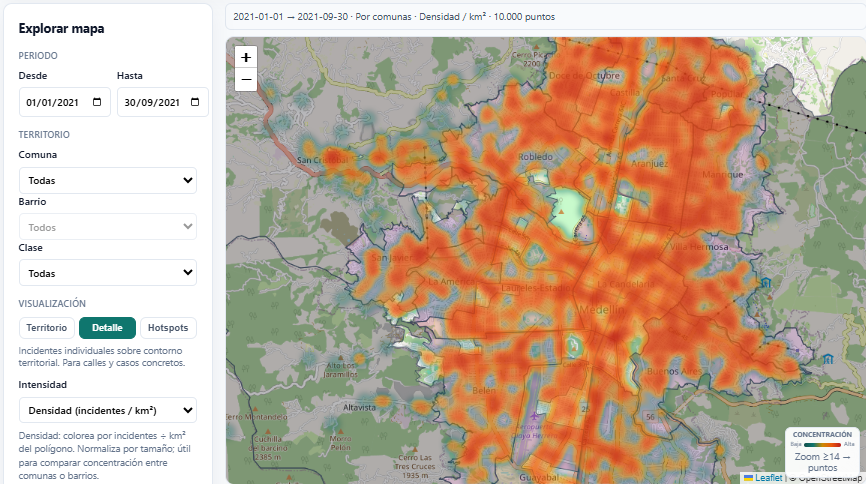
\includegraphics[width=0.88\linewidth]{images/captura_mapa_densidad.png}
	\caption{Mapa analítico — densidad de incidentes por km$^2$ (ene.--sep. 2021, por comunas)}
	\label{fig:captura-mapa-densidad}
\end{figure}

Estos resultados alimentan la priorización territorial (§2) y contextualizan las proyecciones del módulo predictivo.

\subsection{Evaluación del módulo de predicciones}

La evaluación siguió el protocolo metodológico: hold-out de 3 meses, exclusión por defecto de mar--ago 2020 en el ajuste y umbral exploratorio de MAPE hold-out $\leq 20\,\%$. Las tablas siguientes sintetizan los hallazgos principales; el detalle completo permanece en los CSV de \texttt{Fuentes\_viaData/}.

\subsubsection{§1 — Proyección mensual}

En el escenario A (ciudad completa, incidentes, 2018--2021), la Tabla~\ref{tab:resultados-seccion1-a} compara los siete modelos evaluados. \textbf{SARIMA}$(2,1,3)(1,1,1)_{12}$ obtiene el menor MAPE hold-out (\textbf{12,62\,\%}, precisión estimada $\approx 87{,}4\,\%$), por debajo de Poisson y estacional pese a un MAPE in-sample más alto en estos últimos. Este resultado confirma que el criterio hold-out evita sobreajuste: modelos que ajustan bien in-sample no necesariamente generalizan mejor.

\begin{table}[H]
	\centering
	\caption{Proyección mensual de incidentes — escenario A (hold-out 3 meses)}
	\label{tab:resultados-seccion1-a}
	\small
	\begin{tabularx}{\linewidth}{@{}l r r r c@{}}
		\toprule
		\textbf{Modelo} & \textbf{MAPE in-sample (\%)} & \textbf{MAPE hold-out (\%)} & \textbf{Prec. est. (\%)} & \textbf{$\geq 80\,\%$} \\
		\midrule
		SARIMA & 13,14 & \textbf{12,62} & $\approx$87,4 & Sí \\
		Media móvil (3 m) & 6,52 & 15,71 & $\approx$84,3 & Sí \\
		$\mu \pm 3\sigma$ & 11,25 & 17,19 & $\approx$82,8 & Sí \\
		OLS & 11,21 & 18,92 & $\approx$81,1 & Sí \\
		ARIMA & 10,95 & 19,90 & $\approx$80,1 & Límite \\
		Poisson & 8,30 & 22,54 & $\approx$77,5 & No \\
		Estacional & 8,38 & 22,44 & $\approx$77,6 & No \\
		\bottomrule
	\end{tabularx}
\end{table}

La Tabla~\ref{tab:resultados-seccion1-escenarios} resume el mejor modelo por escenario representativo. Para víctimas a nivel ciudad (B) destaca media móvil (14,67\,\%); para víctimas fatales (C), estacional (19,67\,\%); en Castilla (D), media móvil (8,42\,\%); en atropellos (E), Poisson (11,64\,\%). El escenario F, que \textbf{no excluye} COVID del ajuste, degrada SARIMA a 32,87\,\% de MAPE hold-out, reforzando la decisión de exclusión por defecto en la interfaz.

\begin{table}[H]
	\centering
	\caption{Mejor modelo por escenario en proyección mensual (§1)}
	\label{tab:resultados-seccion1-escenarios}
	\small
	\begin{tabularx}{\linewidth}{@{}c l l r@{}}
		\toprule
		\textbf{ID} & \textbf{Contexto} & \textbf{Mejor modelo} & \textbf{MAPE hold-out (\%)} \\
		\midrule
		A & Incidentes ciudad & SARIMA & 12,62 \\
		B & Víctimas ciudad & Media móvil & 14,67 \\
		C & Víctimas fatales ciudad & Estacional & 19,67 \\
		D & Comuna Castilla & Media móvil & 8,42 \\
		E & Clase atropello & Poisson & 11,64 \\
		F & Sin excluir COVID & OLS (11,72); SARIMA (32,87) & Confirma excluir COVID \\
		\bottomrule
	\end{tabularx}
\end{table}

\textbf{Decisión adoptada:} SARIMA$(2,1,3)(1,1,1)_{12}$ para incidentes ciudad; media móvil de tres meses como alternativa interpretable.

Las Figuras~\ref{fig:captura-sarima} y \ref{fig:captura-estacional} muestran la misma configuración de filtros en la interfaz (2018--2021, incidentes ciudad, exclusión mar--ago 2020, hold-out 3 meses) con dos modelos distintos. SARIMA exhibe MAPE hold-out de 12,62\,\% ($\approx 87{,}4\,\%$ de precisión estimada) pese a R$^2$ in-sample bajo; el estacional mejora el ajuste histórico (MAPE 8,38\,\%) pero pierde en la prueba reservada (22,44\,\%), ilustrando por qué la plataforma compara modelos bajo el mismo escenario antes de adoptar uno por defecto.

\begin{figure}[H]
	\centering
	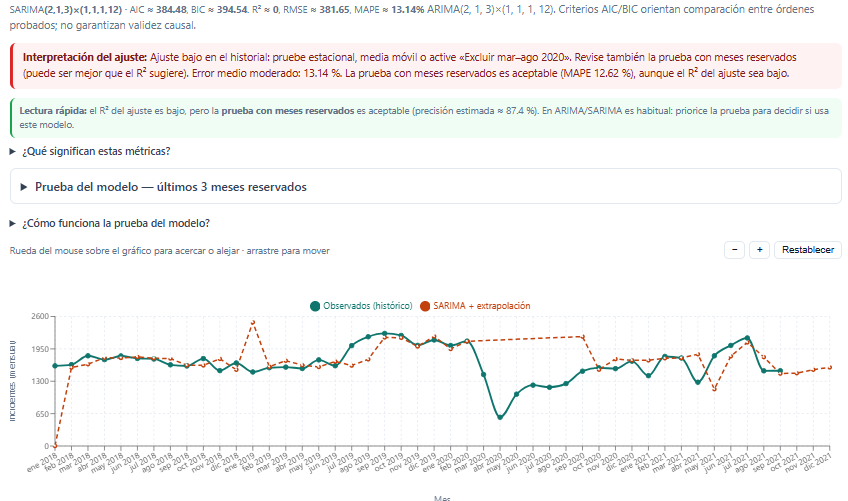
\includegraphics[width=0.92\linewidth]{images/captura_predicciones_sarima.png}
	\caption{Proyección mensual §1 — SARIMA$(2,1,3)(1,1,1)_{12}$, escenario A (hold-out 3 meses)}
	\label{fig:captura-sarima}
\end{figure}

\begin{figure}[H]
	\centering
	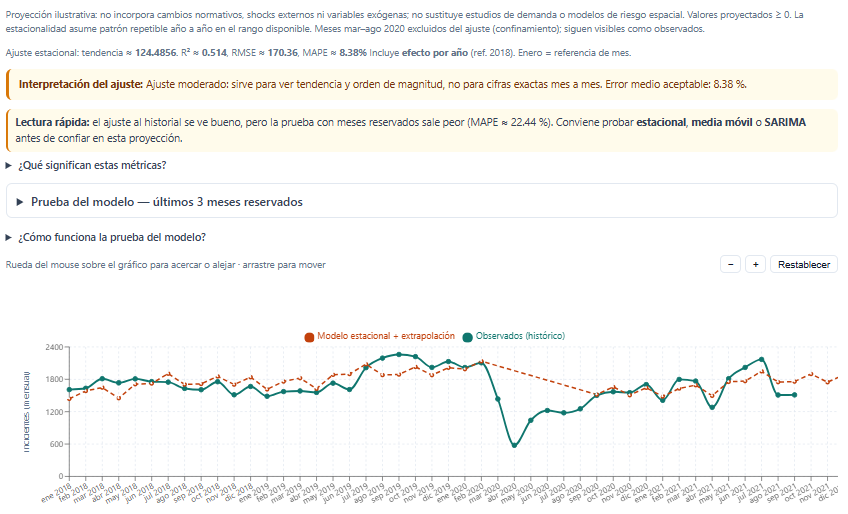
\includegraphics[width=0.92\linewidth]{images/captura_predicciones_estacional.png}
	\caption{Proyección mensual §1 — modelo estacional, mismo escenario A (contraste hold-out)}
	\label{fig:captura-estacional}
\end{figure}

\subsubsection{§2 — Prioridad territorial (índice P05)}

El índice multicriterio P05 (30/15/20/20/15) no entrena modelos predictivos: ordena territorios del periodo filtrado. En escenario A (comunas), \textbf{La Candelaria} lidera con índice \textbf{62,6} y 12\,921 incidentes; la correlación de Spearman entre índice y frecuencia es \textbf{0,8498} y el solapamiento top-5 índice/frecuencia es de 5 territorios, calificando el ranking como \textbf{útil} para priorización. La Figura~\ref{fig:captura-p05} reproduce el ranking en la interfaz, donde La Candelaria lidera por frecuencia, densidad y participación (scores 100 en esos componentes). En barrios (escenario B), el líder por índice es Sin Inf (Robledo), pero el ranking se marca \textbf{parcial} porque el \#1 por índice no coincide con el \#1 por volumen (Spearman 0,9033 sobre top 50 de 270 barrios).

\begin{figure}[H]
	\centering
	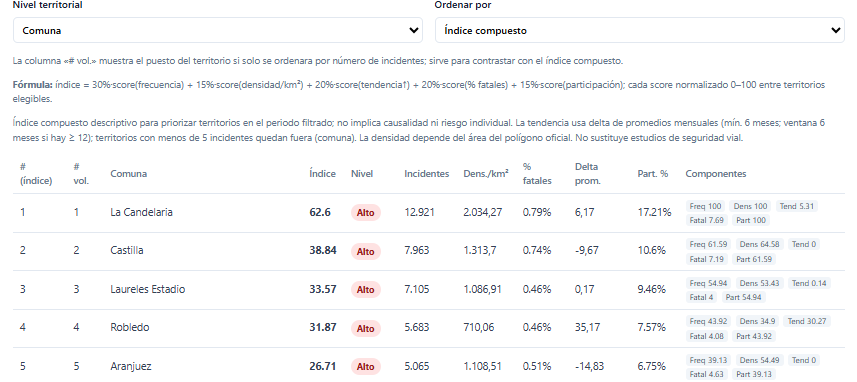
\includegraphics[width=0.95\linewidth]{images/captura_prioridad_p05.png}
	\caption{Prioridad territorial §2 — índice P05 por comuna (escenario A, 2018--2021)}
	\label{fig:captura-p05}
\end{figure}

\subsubsection{§3 — Carga territorial}

En escenario A (comunas), el modelo \textbf{estacional} proyecta la mayor carga en \textbf{La Candelaria} (982,2 incidentes en horizonte de 3 meses) con Spearman carga$\leftrightarrow$frecuencia de \textbf{0,9492} y coherencia con P05 en el territorio líder. El MAPE mediano hold-out territorial ronda \textbf{33\,\%}: las cifras absolutas deben leerse de forma \textbf{comparativa}, no como presupuesto exacto. ARIMA desplaza el líder a Sin Inf (cierre \textbf{parcial}). A nivel barrio, 220 de 270 territorios carecen de proyección individual en el ajuste, por lo que el ranking ciudadano por barrio se reporta como \textbf{parcial}.

\subsubsection{§4 — Proporción de víctimas fatales}

Para el porcentaje mensual de víctimas fatales (escenario A), el modelo \textbf{estacional} alcanza MAPE hold-out de \textbf{21,96\,\%} con R$^2 = 0{,}38$; \textbf{logit con exposición} (20,25\,\%) y \textbf{ratio compuesto} (21,18\,\%) son alternativas viables. OLS, logística, media móvil y ARIMA/SARIMA superan el umbral del 20\,\% en hold-out o presentan R$^2$ cercano a cero, coherente con la volatilidad del indicador. El porcentaje proyectado en horizonte se sitúa en torno a \textbf{0,67\,\%}, cercano al promedio histórico.

\begin{table}[H]
	\centering
	\caption{Proporción de víctimas fatales — escenario A (hold-out 3 meses)}
	\label{tab:resultados-seccion4-a}
	\small
	\begin{tabularx}{\linewidth}{@{}l r r r c@{}}
		\toprule
		\textbf{Modelo} & \textbf{R$^2$} & \textbf{MAPE ajuste (\%)} & \textbf{MAPE hold-out (\%)} & \textbf{Útil} \\
		\midrule
		Estacional & 0,38 & 16,46 & \textbf{21,96} & Sí \\
		Logit con exposición & 0,36 & 15,23 & 20,25 & Sí \\
		Ratio compuesto & 0,38 & 16,13 & 21,18 & Sí \\
		Media móvil & 0,32 & 17,01 & 35,09 & No \\
		OLS / logística & $\approx 0$ & $>$21 & $>$35 & No \\
		\bottomrule
	\end{tabularx}
\end{table}

\subsubsection{§5 — Patrones temporales (P12 y P13)}

Los patrones día$\times$hora heredan el total proyectado de §1 y reparten según pesos históricos con suavizado Laplace. En escenario A, con modelo estacional en §1, el total proyectado a 3 meses es \textbf{5\,530,96} incidentes; la celda líder \textbf{P12} permanece en \textbf{martes 07:00} (69 incidentes proyectados, 1,25\,\% de participación) y el día líder \textbf{P13} es \textbf{martes} (842 incidentes, 15,22\,\%). El Spearman entre ranking observado y proyectado de celdas alcanza \textbf{0,9992}: los modelos mensuales alteran el volumen total pero \textbf{no cambian el patrón relativo} de concentración horaria. Con SARIMA adoptado en §1, el total baja a 4\,572,92 incidentes, manteniendo los mismos líderes temporales.

\subsubsection{Evaluación complementaria $\mu \pm 3\sigma$}

El modelo de línea base $\mu \pm 3\sigma$ proyecta la media histórica con bandas de control. En escenario A (§1), la media es 1\,753,4 incidentes/mes ($\sigma = 247{,}6$); el 100\,\% de los meses de ajuste caen dentro de $\mu \pm 3\sigma$ y el MAPE hold-out es 17,19\,\%. No reemplaza a SARIMA en ciudad, pero aporta un contraste didáctico y bandas de control interpretables.

\subsection{Validación técnica del software}

La validación técnica se ejecutó mediante la suite \texttt{pytest} con \texttt{pytest-django} sobre las aplicaciones \texttt{dashboard}, \texttt{agent}, \texttt{accounts} y \texttt{reports}, usando configuración de prueba con SQLite en memoria. La ejecución completa finalizó en verde, cubriendo endpoints de KPIs, predicciones, autenticación JWT, herramientas del asistente y generación de payloads de reportes. Complementariamente, el comando \texttt{manage.py check\_postgis} verifica la disponibilidad de extensiones espaciales en despliegues con PostgreSQL.

Esta evidencia respalda el objetivo específico de validar desempeño y seguridad del software. No sustituye una auditoría de carga en producción, pero confirma que los módulos críticos del backend responden de forma coherente bajo pruebas automatizadas reproducibles.

\subsection{Síntesis de resultados}

En conjunto, ViaData — Medellín cumple los objetivos planteados y entrega un instrumento geoespacial consultable sobre datos Mede. La analítica descriptiva identifica concentraciones territoriales y temporales estables (La Candelaria; martes 07:00). El módulo predictivo adopta modelos transparentes con validación hold-out: SARIMA para incidentes ciudad, estacional para carga territorial y proporción de fatales, e índice P05 fijo para priorización inmediata. Las limitaciones de precisión territorial (MAPE mediano $\approx 33\,\%$), la volatilidad del \% de fatales y el alcance parcial en barrios se discuten en la sección de discusión.


\section{DISCUSIÓN}
\subsection{Interpretación de los resultados}

Los resultados de la sección anterior confirman que ViaData — Medellín cumple los objetivos planteados y entrega evidencia numérica reproducible sobre datos Mede. Más allá del cumplimiento técnico, la lectura analítica del sistema sugiere tres mensajes centrales para la gestión de la accidentalidad urbana.

En primer lugar, la \textbf{concentración territorial y temporal} no es aleatoria: La Candelaria lidera múltiples rankings y el patrón martes 07:00 se mantiene estable al proyectar, en línea con estudios que vinculan SIG y focalización territorial en seguridad vial \cite{xu2022,monar2025}. Esto respalda el uso del tablero y el mapa como instrumentos de diagnóstico antes de cualquier proyección.

En segundo lugar, el módulo predictivo \textbf{no reemplaza} el análisis descriptivo: el índice P05 (§2) resume el periodo ya observado, mientras que §1 y §3 orientan escenarios futuros con lógicas distintas. La coherencia entre ambos ---La Candelaria líder en prioridad y en carga proyectada en comunas--- refuerza la interpretación territorial, pero no debe confundirse con causalidad ni con certeza presupuestal.

En tercer lugar, la \textbf{validación hold-out} resultó más informativa que el ajuste in-sample para seleccionar modelos en series mensuales perturbadas por la pandemia, coherente con la literatura de conteos y series temporales en accidentalidad, donde la estacionalidad y los shocks estructurales condicionan el desempeño \cite{lugo2025,parraga2024}.

\subsection{Contingencia del desempeño predictivo según escenario}

Un hallazgo relevante de la evaluación es que \textbf{no existe un modelo único óptimo} para todos los contextos analíticos. La efectividad de OLS, estacional, Poisson, media móvil, $\mu \pm 3\sigma$, ARIMA o SARIMA depende del \textbf{escenario} definido por el usuario: variable objetivo (incidentes, víctimas o fatales), alcance territorial (ciudad, comuna, barrio, clase de incidente), longitud del periodo de ajuste y decisión de excluir o no los meses de confinamiento de 2020.

La Tabla~\ref{tab:resultados-seccion1-escenarios} lo ilustra con claridad. SARIMA obtiene el mejor hold-out para incidentes a nivel ciudad cuando hay al menos 24 meses útiles y se excluye COVID del ajuste (12,62\,\% MAPE). Sin embargo, para víctimas totales gana la media móvil (14,67\,\%), para víctimas fatales el estacional (19,67\,\%), en Castilla la media móvil (8,42\,\%) y en atropellos Poisson (11,64\,\%). Cuando COVID permanece en el ajuste (escenario F), SARIMA se degrada a 32,87\,\% de MAPE hold-out, mientras modelos más simples conservan errores menores.

Este patrón tiene implicaciones metodológicas y prácticas. Las Figuras~\ref{fig:captura-sarima-config} y \ref{fig:captura-estacional} del capítulo de resultados muestran, bajo idénticos filtros (escenario A), cómo un modelo con mejor ajuste in-sample puede perder frente a SARIMA en la prueba reservada:

\begin{itemize}
	\item \textbf{Selección condicionada:} elegir modelo solo por R$^2$ o MAPE in-sample puede sobrevalorar Poisson y estacional en §1 (8,3--8,4\,\% in-sample frente a 22\,\% hold-out), ilustrando el riesgo de sobreajuste que la validación reservada mitiga.
	\item \textbf{Requisitos de datos:} rangos cortos (6--12 meses) impiden o inestabilizan ARIMA/SARIMA; en esos cortes predominan media móvil, $\mu \pm 3\sigma$ o modelos parsimoniosos, no la especificación adoptada para ciudad.
	\item \textbf{Granularidad territorial:} a nivel comuna algunos territorios proyectan con MAPE aceptable; a nivel barrio, 220 de 270 carecen de serie suficiente en §3, lo que limita la confianza en cifras absolutas y obliga a priorizar \textbf{rankings} sobre magnitudes puntuales.
	\item \textbf{Tipo de variable:} el porcentaje de víctimas fatales es más volátil que los conteos mensuales; allí el estacional supera a SARIMA/ARIMA, que exhiben MAPE hold-out superiores al 28\,\%.
\end{itemize}

Por ello, la interfaz de predicciones no impone un modelo cerrado de forma silenciosa: expone la \textbf{comparación multi-modelo y multi-escenario} y documenta la decisión adoptada por defecto (SARIMA ciudad incidentes; estacional en carga y \% fatales). El valor institucional del sistema reside tanto en la proyección puntual como en permitir al analista contrastar \textit{qué} cambia al variar territorio, periodo o tratamiento del shock COVID. Las proyecciones deben leerse como \textbf{escenarios orientativos} bajo estabilidad del patrón histórico filtrado, no como pronósticos únicos \cite{oms2024}.

\subsection{Coherencia entre bloques analíticos}

La cadena §1$\rightarrow$§5 muestra que el modelo mensual elegido altera el \textbf{volumen} proyectado pero no el \textbf{orden relativo} del patrón día$\times$hora (Spearman $\approx 0{,}999$). Esto es consistente con un diseño en dos pasos: primero se estima el total del horizonte; luego se reparte según pesos históricos con suavizado Laplace. Para planificación operativa ---franjas horarias de control o campañas--- el mensaje útil es la \textbf{persistencia del patrón}, más que la cifra exacta del mes proyectado.

Entre §2 y §3, P05 mide prioridad del \textit{pasado reciente} con ponderación multicriterio fija; la carga territorial proyecta el \textit{futuro} con modelos por territorio. Su coincidencia en La Candelaria refuerza la focalización, pero el índice puede destacar territorios con alta densidad o tendencia aunque no lideren volumen bruto ---como ocurre en barrios, donde Sin Inf (Robledo) encabeza P05 sin ser el de mayor frecuencia absoluta en el top general---. Esta distinción es deseable: priorización y proyección responden preguntas complementarias.

\subsection{Limitaciones del estudio}

\begin{table}[H]
	\centering
	\caption{Limitaciones principales de ViaData — Medellín}
	\label{tab:limitaciones}
	\small
	\begin{tabularx}{\linewidth}{@{}l X@{}}
		\toprule
		\textbf{Área} & \textbf{Limitación} \\
		\midrule
		Causalidad & No se incorporan variables exógenas (clima, políticas, cambios normativos, intervenciones viales) \\
		COVID-19 & Shock estructural; la exclusión parcial del ajuste no elimina el fenómeno del periodo observado \\
		Datos & ETL manual; periodo fijo aproximado 2014--2021; dependencia de calidad y cobertura Mede \\
		Territorio fino & Proyección barrial limitada por volumen insuficiente en muchos barrios (§3 parcial) \\
		Cifras absolutas & MAPE territorial mediano $\approx 33\,\%$; rankings más confiables que magnitudes exactas \\
		Patrones §5 & Asumen estacionariedad del reparto día$\times$hora respecto al periodo filtrado \\
		Alcance omitido & Sin ranking por vía o punto crítico (Mede no alimenta esos catálogos); sin ML espacial avanzado \\
		Asistente IA & Respuestas dependen de herramientas API; tier gratuito Gemini con restricciones de uso \\
		Inferencia individual & No se estima probabilidad personal de sufrir un siniestro \\
		\bottomrule
	\end{tabularx}
\end{table}

La calidad del dato administrativo sigue siendo condición previa para cualquier política basada en evidencia \cite{oviedo2025,atancuri2024}. El indicador G03 ayuda a visibilizar discrepancias entre territorio declarado y espacial, pero no corrige automáticamente errores de georreferenciación en la fuente.

\subsection{Amenazas a la validez}

\textbf{Validez interna:} el esquema hold-out reduce el sobreajuste en §1 y §4; §2 y §5 emplean reglas fijas documentadas (índice P05 y reparto histórico), lo que limita el riesgo de optimización ad hoc. No obstante, la elección de excluir mar--ago 2020 es una decisión de diseño que altera el ranking de modelos y debe explicitarse en cada consulta.

\textbf{Validez externa:} los hallazgos son válidos para Medellín y el periodo Mede cargado. La generalización a otras ciudades o a periodos posteriores requiere recalibración del ETL, nuevos polígonos y reevaluación hold-out.

\textbf{Validez de constructo:} el umbral exploratorio de ``precisión $\approx 80\,\%$'' corresponde a MAPE hold-out $\leq 20\,\%$, no a R$^2 \geq 0{,}80$. En series mensuales con estacionalidad y confinamiento, exigir R$^2$ elevado habría descartado modelos útiles en hold-out (SARIMA ciudad exhibe R$^2$ in-sample bajo pese a MAPE hold-out competitivo).

\subsection{Utilidad para la toma de decisiones}

A pesar de las limitaciones, el sistema aporta valor en tres frentes alineados con el objetivo general: \textbf{(i)} visualización integrada de accidentalidad georreferenciada; \textbf{(ii)} segmentación por territorio, tiempo, clase y gravedad; y \textbf{(iii)} escenarios predictivos comparables bajo criterios explícitos. Para actores institucionales, la recomendación de uso es:

\begin{enumerate}
	\item Explorar primero tablero y mapa para caracterizar el periodo de interés.
	\item Aplicar P05 para priorización territorial del pasado reciente.
	\item Contrastar al menos dos escenarios predictivos (periodo, COVID, territorio) antes de adoptar una proyección.
	\item Interpretar §3 y §5 en clave de \textbf{ranking y patrón}, no de cifra exacta.
	\item Documentar filtros y modelo elegido al exportar reportes.
\end{enumerate}

En síntesis, la efectividad de cada modelo predictivo es \textbf{contingente al escenario analítico}. ViaData — Medellín materializa esa contingencia en la interfaz y en la evaluación reproducible, ofreciendo transparencia metodológica en lugar de un único número cerrado. Las conclusiones y el trabajo futuro derivan de este balance entre utilidad exploratoria y límites del dato y del alcance del proyecto.



\section{CONCLUSIONES}
El presente trabajo de grado desarrolló e implementó \textbf{ViaData — Medellín}, instrumento virtual geoespacial orientado al análisis y la proyección exploratoria de la accidentalidad vial en Medellín a partir de datos abiertos Mede. A continuación se sintetizan las conclusiones derivadas del diseño, la implementación, la evaluación numérica y la validación técnica del sistema, en correspondencia con el objetivo general y los objetivos específicos planteados.

En relación con el \textbf{objetivo general}, se logró construir una plataforma web que integra visualización interactiva, segmentación territorial y temporal, e indicadores y modelos estadísticos transparentes para apoyar la lectura del fenómeno y la discusión de escenarios en seguridad vial. El tablero y el mapa permiten consulta pública de KPIs, series, matrices día$\times$hora y capas geoespaciales; el módulo de predicciones, los reportes y el asistente conversacional amplían esa capacidad para perfiles analista y administrador, con trazabilidad entre la interfaz y el motor de cálculo del backend.

Respecto al \textbf{objetivo específico 1} (arquitectura y modelo de datos geoespacial), se adoptó una arquitectura monolítica en Django con API REST, autenticación JWT y frontend React, apoyada en PostgreSQL/PostGIS. El flujo ETL reproducible ---centralizado en \texttt{mede\_limpieza.py} y documentado en manuales de carga--- transforma el Excel Mede en una base relacional con incidentes, víctimas, catálogos y geometrías, habilitando consultas espaciales y el contraste entre modo territorio \textit{registro} y \textit{espacial}.

En cuanto al \textbf{objetivo específico 2} (módulos de análisis estadístico), el sistema calcula indicadores descriptivos y diagnósticos (densidad G01--G02, calidad G03, rankings, matrices temporales) y un módulo predictivo estructurado en cinco bloques (§1--§5). La evaluación cerrada y el caso de estudio escenario A adoptaron: \textbf{SARIMA}$(2,1,3)(1,1,1)_{12}$ para proyección mensual de incidentes a nivel ciudad (MAPE hold-out 12,62\,\%); \textbf{índice P05} para priorización territorial del periodo; \textbf{modelo estacional} para ranking de carga futura por comuna; \textbf{logit con exposición} para la proporción de víctimas fatales (MAPE hold-out 20,25\,\%); y \textbf{reparto histórico} con suavizado Laplace para patrones día$\times$hora y día de la semana, heredando el total de §1.

Frente al \textbf{objetivo específico 3} (tablero de monitoreo y diagnóstico), la ruta \texttt{/tablero} materializa la evolución mensual, la comparación interanual y la distribución por territorio, día y hora. El mapa analítico complementa esa lectura con puntos, densidad, coroplética y concentraciones espaciales. Los resultados confirman concentraciones recurrentes ---La Candelaria en volumen e índice P05; martes 07:00 en patrones temporales--- que orientan la focalización territorial.

En el \textbf{objetivo específico 4} (validación técnica), la suite \texttt{pytest} sobre las aplicaciones críticas del backend finalizó en verde, y el módulo de predicciones cuenta con evaluación reproducible en CSV y scripts documentados. El criterio de validación predictiva basado en \textit{hold-out} (MAPE $\leq 20\,\%$ como umbral exploratorio) resultó más informativo que exigir R$^2 \geq 0{,}80$ en series mensuales con estacionalidad y confinamiento COVID.

Además de los objetivos formales, se entregaron componentes complementarios ---mapa analítico, reportes imprimibles, asistente con Gemini y gestión de usuarios--- que facilitan la operación y la comunicación de hallazgos sin alterar la formulación académica del proyecto.

Desde el plano analítico, las conclusiones centrales del estudio son las siguientes:

\begin{enumerate}
	\item Los datos abiertos Mede, depurados y cargados con reglas únicas, permiten sostener un instrumento geoespacial consultable sobre del orden de 160\,000+ incidentes georreferenciados en el periodo cargado (aprox. 2014--2021).
	\item La analítica descriptiva y geoespacial evidencia que la siniestralidad se concentra en corredores y comunas del valle urbano, con patrones temporales persistentes que complementan la lectura por volumen bruto.
	\item \textbf{No existe un modelo predictivo único óptimo} para todos los escenarios: la efectividad depende de la variable, el territorio, la longitud del periodo y el tratamiento del shock COVID; la interfaz expone esa contingencia mediante comparación multi-modelo bajo filtros explícitos.
	\item El hold-out discrimina mejor que el ajuste in-sample entre modelos parsimoniosos y especificaciones más flexibles; Poisson y estacional pueden ajustar bien el historial y perder en meses reservados, mientras SARIMA lidera en incidentes ciudad bajo escenario A.
	\item Las proyecciones son \textbf{herramientas exploratorias} para priorización y planificación: apoyan la discusión de escenarios bajo estabilidad del patrón histórico filtrado, pero no establecen causalidad ni estiman riesgo individual \cite{oms2024,parraga2024}.
\end{enumerate}

En conjunto, ViaData — Medellín demuestra que es viable articular ingeniería de software, sistemas de información geográfica y ciencia de datos en un mismo entorno orientado a la seguridad vial urbana, con modelos interpretables y evaluación documentada \cite{lugo2025,monar2025}. Las limitaciones de generalización temporal, precisión territorial fina, ausencia de variables exógenas y alcance omitido (ranking por vía, ingesta automática, ML espacial avanzado) se abordaron en la discusión y orientan las líneas de trabajo futuro de la siguiente sección.


\section{TRABAJO FUTURO}
\subsection{Ampliación de datos y gobernanza de la información}

La versión actual de ViaData — Medellín opera sobre un periodo Mede aproximado de 2014--2021 y un flujo ETL \textbf{manual pero reproducible}. Como línea prioritaria de trabajo futuro se plantea la \textbf{ingesta automática o programada} de nuevas versiones del conjunto Mede, con validación de esquema, alertas de calidad y versionado de cargas. Complementariamente, la \textbf{extensión temporal} del repositorio permitiría recalibrar modelos predictivos, reevaluar hold-out y contrastar tendencias post-2021, condicionado a la disponibilidad y consistencia de datos abiertos actualizados por la institución \cite{atancuri2024,oviedo2025}.

En paralelo, conviene fortalecer la gobernanza del dato: trazabilidad de transformaciones, metadatos de cada carga y documentación de cambios en catálogos o definiciones operativas, de modo que las proyecciones futuras mantengan comparabilidad con las evaluaciones ya cerradas.

\subsection{Indicadores y análisis geoespacial omitidos}

Durante el cronograma del proyecto se omitieron deliberadamente funcionalidades ligadas a catálogos que Mede no alimenta en la versión cargada:

\begin{itemize}
	\item \textbf{P11 — ranking por vía o punto crítico}, por ausencia de registros en tablas \texttt{via} y \texttt{punto\_critico}.
	\item \textbf{G04 — análisis por buffer de punto crítico}, mientras la tabla de puntos críticos permanezca vacía.
	\item \textbf{G05 — filtro por bounding box en mapa}, considerado redundante frente a filtros por comuna y barrio.
\end{itemize}

Una extensión natural del sistema consiste en incorporar estos indicadores \textbf{si la fuente institucional publica geometrías o identificadores de corredores e intersecciones} de forma estructurada, lo que habilitaría focalizar intervenciones en glorietas, tramos viales o nodos de alta siniestralidad ---línea de investigación coherente con estudios de puntos críticos en Medellín \cite{viveros2022,xu2022}.

Asimismo, profundizar el contraste entre modo \textit{registro} y modo \textit{espacial} (indicador G03) con reportes periódicos de calidad cartográfica aportaría evidencia para mejorar la georreferenciación en la captura administrativa.

\subsection{Modelos predictivos y evaluación}

La evaluación cerrada priorizó modelos \textbf{transparentes y comparables} (OLS, estacional, Poisson, media móvil, $\mu \pm 3\sigma$, ARIMA/SARIMA) y demostró que el desempeño depende del escenario analítico. Trabajo futuro en esta línea podría incluir:

\begin{itemize}
	\item \textbf{Modelos jerárquicos o bayesianos} para series territoriales con pocos datos por barrio, mitigando la limitación actual en que 220 de 270 barrios carecen de proyección individual en §3.
	\item \textbf{P15 — aprendizaje automático espacial} (por ejemplo, gradient boosting o modelos de conteo espacio-temporales), evaluados siempre con hold-out y sin sustituir la trazabilidad de las formulaciones actuales.
	\item \textbf{Variables exógenas} (meteorología, intervenciones viales, cambios normativos) para acercar las proyecciones a escenarios contrafactuales, sin pretender inferencia causal plena desde el registro administrativo.
	\item \textbf{Reevaluación periódica} del ranking de modelos al incorporar nuevos meses, automatizando los scripts \texttt{llenar\_evaluacion\_seccion*.py} en un pipeline de CI.
\end{itemize}

Se mantiene como criterio que cualquier modelo nuevo deba superar o complementar el protocolo MAPE hold-out $\leq 20\,\%$ antes de adoptarse como predeterminado en producción.

\subsection{Plataforma, despliegue y adopción institucional}

En el plano de ingeniería de software, extensiones viables incluyen:

\begin{itemize}
	\item \textbf{Generación de PDF en servidor} (Puppeteer, WeasyPrint u equivalente) como alternativa a la impresión nativa del navegador.
	\item \textbf{Activación del rol autoridad} reservado en el esquema de permisos, con flujos de aprobación o publicación de reportes oficiales.
	\item \textbf{Integración con tableros institucionales} o APIs de movilidad urbana, si la entidad dispone de canales de intercambio seguros.
	\item \textbf{Pruebas de carga y despliegue productivo} (contenedorización, respaldos, monitoreo) que exceden el alcance de validación con \texttt{pytest} del trabajo de grado.
\end{itemize}

El asistente conversacional basado en Gemini podría evolucionar hacia un catálogo ampliado de herramientas, auditoría de consultas y, en entornos institucionales, despliegue con políticas de privacidad y retención distintas al tier gratuito actual.

\subsection{Síntesis de prioridades}

En síntesis, las prioridades de trabajo futuro se ordenan así: \textbf{(1)} actualizar y automatizar el dato; \textbf{(2)} incorporar indicadores viales y puntos críticos si la fuente lo permite; \textbf{(3)} ampliar el repertorio predictivo con evaluación hold-out rigurosa, especialmente en barrios; y \textbf{(4)} madurar el despliegue y la adopción institucional del instrumento. La Figura~\ref{fig:flujo-trabajo-futuro} resume el flujo propuesto y las dependencias entre fases. Estas líneas prolongan el equilibrio alcanzado en ViaData — Medellín entre utilidad exploratoria, transparencia metodológica y reconocimiento explícito de limitaciones \cite{lugo2025,monar2025}.

\begin{figure}[H]
	\centering
	\resizebox{0.88\linewidth}{!}{%
	\begin{tikzpicture}[
		node distance=0.55cm,
		box/.style={draw, rounded corners, align=center, font=\scriptsize, inner sep=4pt, minimum width=6.2cm},
		dec/.style={draw, diamond, aspect=2.2, align=center, font=\scriptsize, inner sep=1pt, minimum width=2.8cm},
		end/.style={draw, rounded corners, align=center, font=\scriptsize, inner sep=4pt, minimum width=5.6cm, fill=gray!12},
		arr/.style={-{Stealth[length=1.8mm]}, thick},
		skip/.style={-{Stealth[length=1.8mm]}, thick, dashed}
	]
		\node[box, fill=blue!8] (act) {Estado actual: ViaData — Medellín (2014--2021, ETL manual reproducible)};
		\node[box, fill=green!12, below=of act] (p1) {\textbf{(1) Datos y gobernanza}\\Ingesta automática · validación de esquema · versionado · extensión temporal · metadatos};
		\node[dec, below=of p1] (cond) {¿Mede publica\\vías y puntos críticos?};
		\node[box, fill=yellow!18, below left=0.9cm and 0.2cm of cond] (p2) {\textbf{(2) Indicadores geoespaciales}\\P11 ranking vial · G04 buffer · G05 bbox · contraste registro/espacial};
		\node[box, fill=orange!15, below=1.35cm of cond] (p3) {\textbf{(3) Modelos predictivos}\\Jerárquicos/bayesianos · P15 ML espacial · variables exógenas · pipeline CI · MAPE hold-out $\leq 20\,\%$};
		\node[box, fill=violet!10, below=of p3] (p4) {\textbf{(4) Plataforma e institucionalización}\\PDF en servidor · rol autoridad · APIs · despliegue productivo · asistente ampliado};
		\node[end, below=of p4] (fin) {Sistema actualizado, trazable y orientado a adopción institucional};

		\draw[arr] (act) -- (p1);
		\draw[arr] (p1) -- (cond);
		\draw[arr] (cond) -- node[above left, font=\tiny, sloped] {sí} (p2);
		\draw[arr] (p2) -- (p3);
		\draw[arr] (cond) -- node[above right, font=\tiny, sloped] {no} (p3);
		\draw[arr] (p3) -- (p4);
		\draw[arr] (p4) -- (fin);
	\end{tikzpicture}%
	}
	\caption{Diagrama de flujo de las líneas de trabajo futuro propuestas para ViaData — Medellín}
	\label{fig:flujo-trabajo-futuro}
\end{figure}


%% salto de pagina
%\noindent \begin{center}
%\cleardoublepage{}
%\par\end{center}
%
%% publicar:  comentar layout 
%\layout*
%\noindent \begin{center}
%\cleardoublepage{}
%\par\end{center}
%\medskip


% ver [doc-434]. se cambia a español para que los meses y las abreviacion sean en español. 
\selectlanguage{spanish}
% necesario porque el paquete  titlesec cambiar comportamientos internos de las secciones.
% Por tal motivo el anchor de los hyperref estan corruptos. Es necesario agregar
% Phantomsection antes de una adicion manual a la tabla de contenido [heading=bibintoc]
\phantomsection 
\printbibliography[heading=bibintoc, title={REFERENCIAS}]
% ver [doc-434]. se coloca de nuevo en ingles. 
\selectlanguage{english}

\section{ANEXOS}
\subsection{Anexo A — Diagrama entidad-relación del modelo de datos}

El modelo relacional de ViaData — Medellín organiza el dominio de accidentalidad en tablas de hechos (\texttt{incidente}, \texttt{victima}), catálogos descriptivos (sexo, grupo de edad, condición, gravedad, clase de incidente), territorio (comuna, barrio) y tablas opcionales para infraestructura vial (\texttt{via}, \texttt{punto\_critico}), previstas en el esquema pero sin población desde Mede en la versión evaluada. La Figura~\ref{fig:esquema-bd} resume las relaciones principales; el DDL completo se incluye en el Anexo~B.

Las geometrías oficiales de comunas y barrios se gestionan en PostGIS (scripts \texttt{001}--\texttt{006} del pipeline de carga) y complementan las claves foráneas declarativas del registro Mede. El módulo de autenticación extiende \texttt{auth\_user} de Django mediante \texttt{perfil\_usuario} y la tabla \texttt{rol}.

\begin{figure}[H]
	\centering
	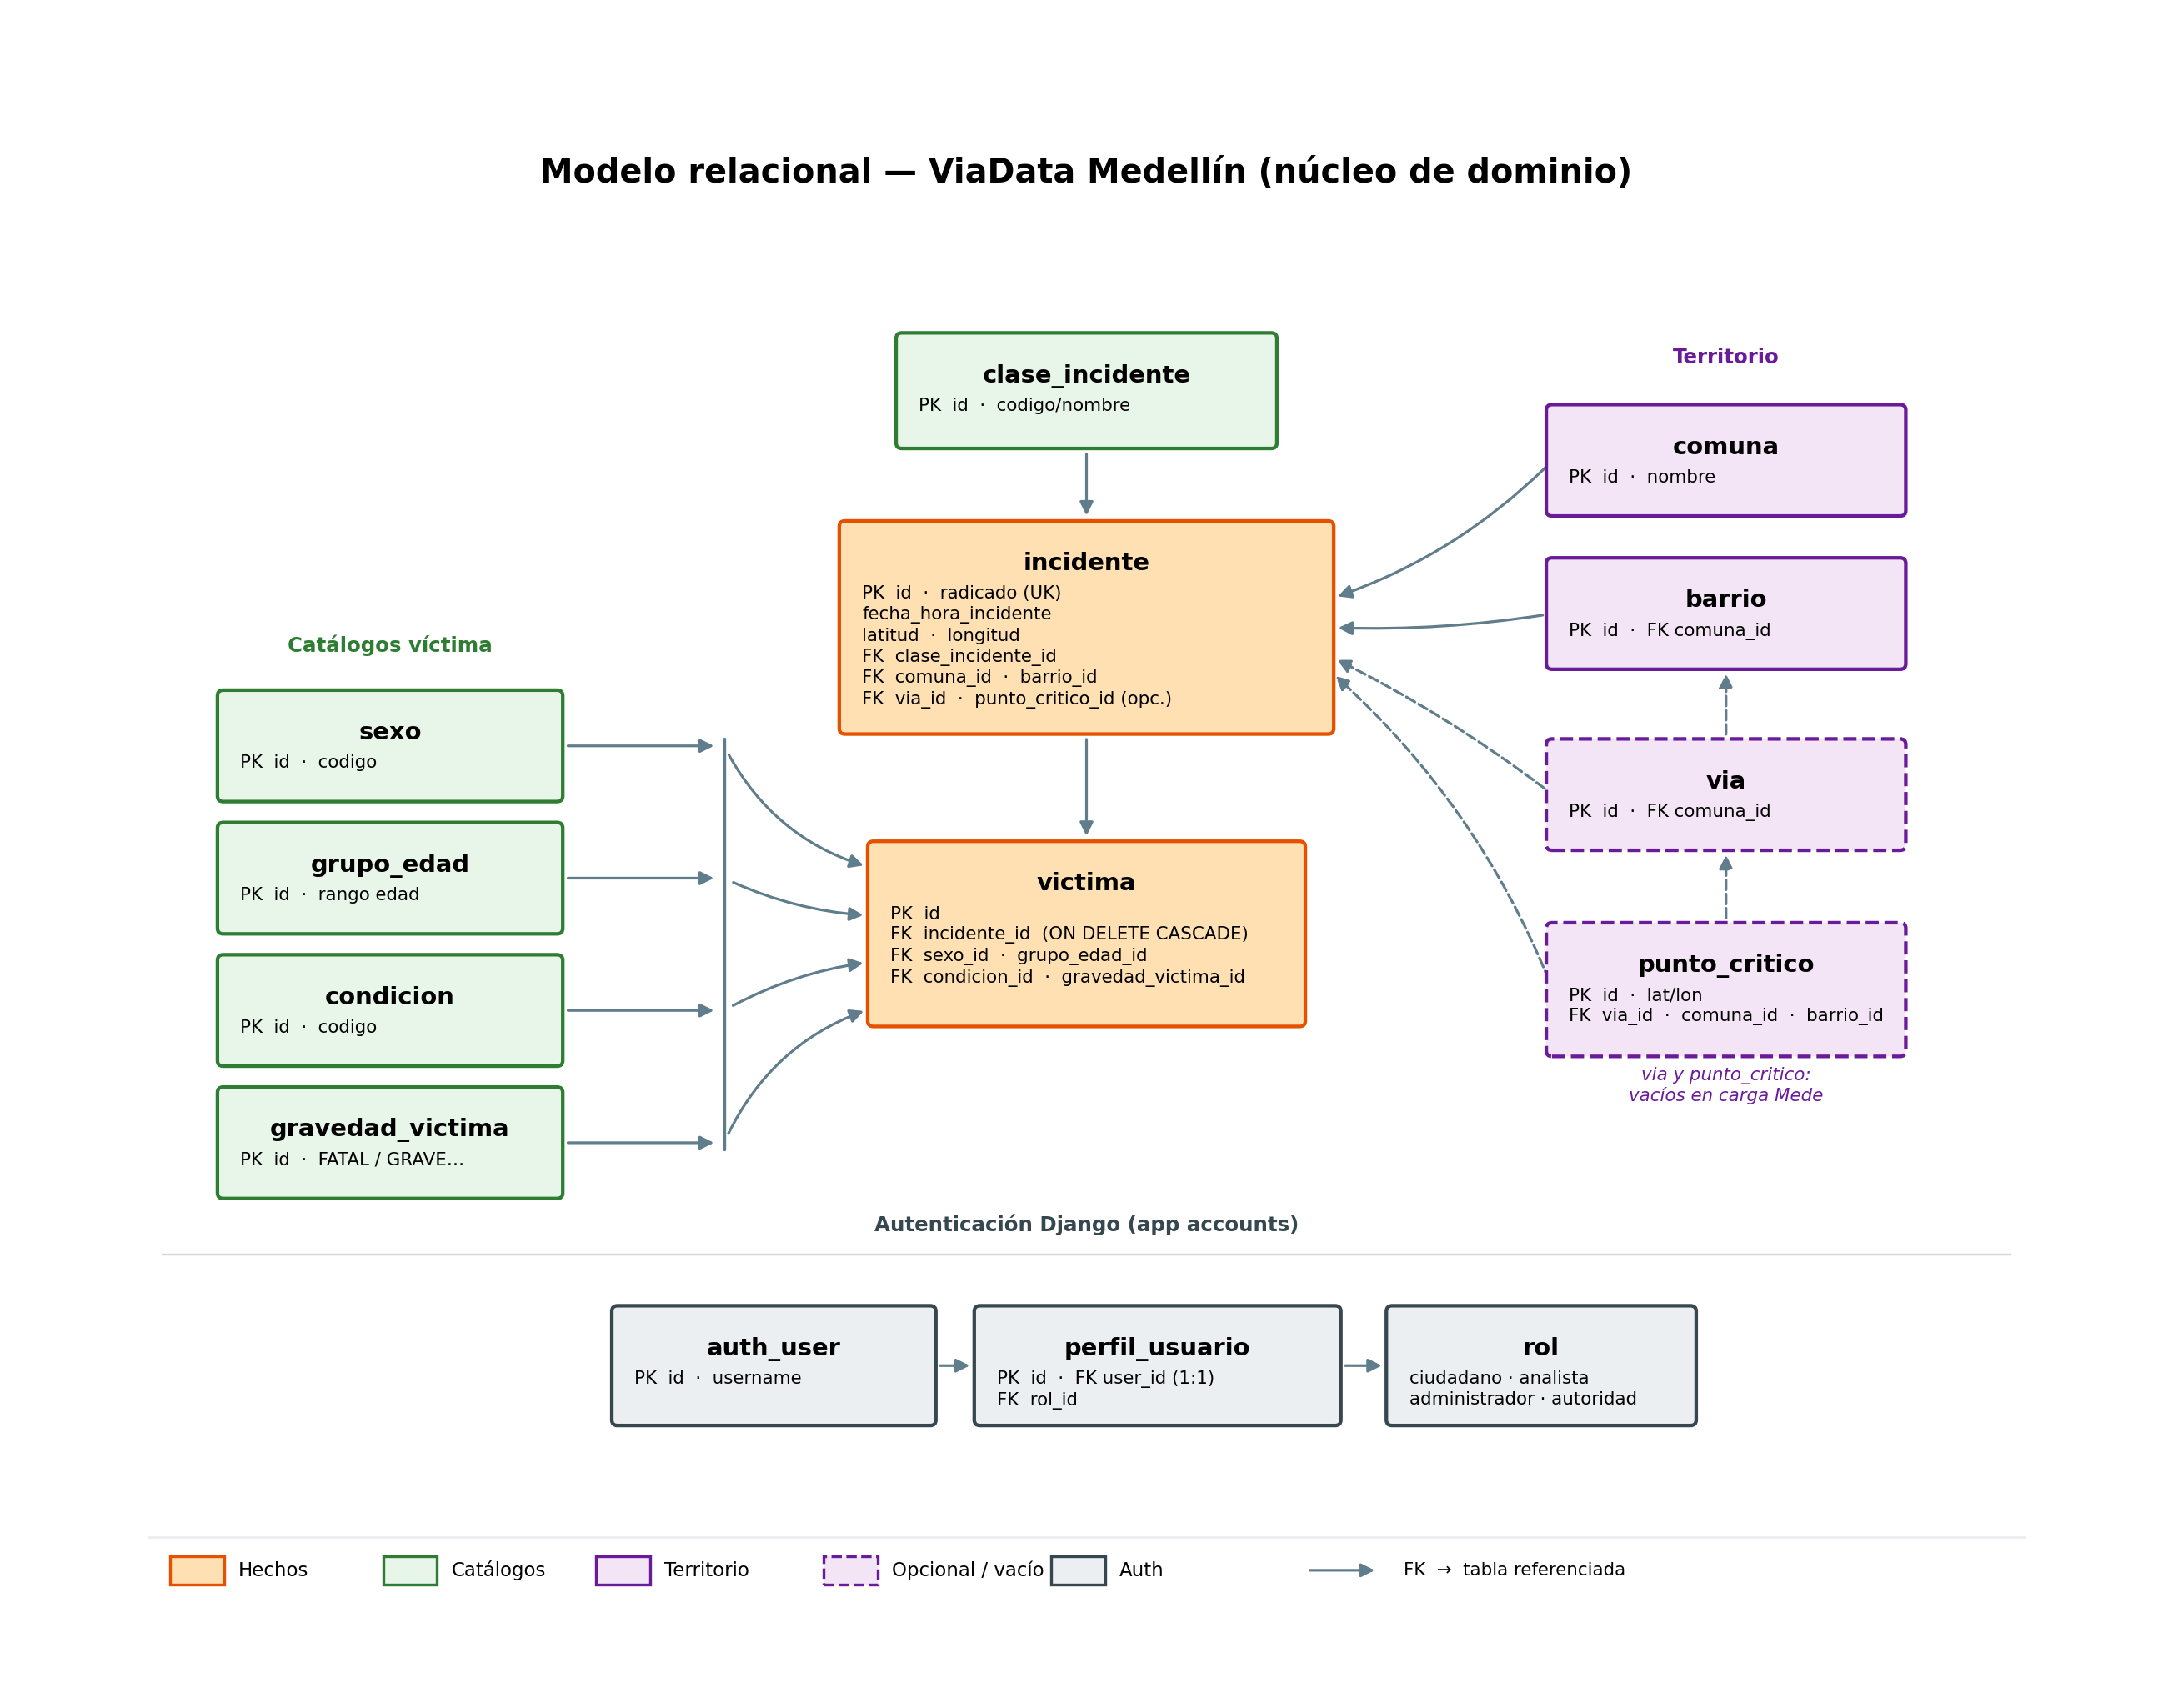
\includegraphics[width=0.98\linewidth]{images/fig_esquema_bd.png}
	\caption{Diagrama entidad-relación simplificado del núcleo de dominio}
	\label{fig:esquema-bd}
\end{figure}

\subsection{Anexo B — Esquema SQL de la base de datos}

El listado siguiente corresponde al archivo \texttt{Fuentes\_viaData/esquema\_base\_datos.sql}, que define catálogos, tablas principales, índices, vistas analíticas (\texttt{vista\_incidentes\_completa}, \texttt{vista\_estadisticas\_victimas}) y el bloque de autenticación Django (\texttt{auth\_user}, \texttt{perfil\_usuario}, \texttt{rol}, sesiones y permisos).

\begin{minted}[fontsize=\scriptsize,breaklines,breakanywhere]{sql}
-- Tablas principales (extracto)
CREATE TABLE incidente (
    id SERIAL PRIMARY KEY,
    radicado VARCHAR(50) UNIQUE NOT NULL,
    fecha_hora_incidente TIMESTAMP NOT NULL,
    clase_incidente_id INTEGER REFERENCES clase_incidente(id),
    latitud DECIMAL(10, 8),
    longitud DECIMAL(11, 8),
    comuna_id INTEGER REFERENCES comuna(id),
    barrio_id INTEGER REFERENCES barrio(id),
    via_id INTEGER REFERENCES via(id),
    punto_critico_id INTEGER REFERENCES punto_critico(id)
);

CREATE TABLE victima (
    id SERIAL PRIMARY KEY,
    incidente_id INTEGER NOT NULL REFERENCES incidente(id) ON DELETE CASCADE,
    sexo_id INTEGER REFERENCES sexo(id),
    grupo_edad_id INTEGER REFERENCES grupo_edad(id),
    condicion_id INTEGER REFERENCES condicion(id),
    gravedad_victima_id INTEGER REFERENCES gravedad_victima(id)
);
\end{minted}

El script íntegro incluye además datos semilla de catálogos, índices de consulta frecuente y comentarios de tablas de usuario. Se recomienda consultar el archivo fuente en el repositorio del proyecto para despliegues y migraciones.

\subsection{Anexo C — Manual de carga de datos (ETL Mede)}

La ingesta reproducible sigue el flujo documentado en \texttt{MANUAL\_CARGA\_DATOS\_BD.md}:

\begin{enumerate}
	\item Depuración del Excel con \texttt{mede\_limpieza.depurar\_mede()} (reglas únicas de calidad).
	\item Exportación a \texttt{Mede\_Victimas\_inci\_depurado.csv}.
	\item Carga idempotente con \texttt{carga\_mede\_pgadmin.sql}.
	\item Ejecución de scripts PostGIS y carga de polígonos (\texttt{cargar\_poligonos\_medellin}, \texttt{actualizar\_territorio\_espacial}).
	\item Verificación de conteos y del indicador G03 en la interfaz.
\end{enumerate}

Principio de diseño: toda regla de limpieza reside en \texttt{mede\_limpieza.py}; EDA, pipeline guiado y memoria de grado deben importar la misma lógica para garantizar reproducibilidad.

\subsection{Anexo D — Manual de instalación y ejecución}

Para replicar el entorno de desarrollo o demostración, \texttt{MANUAL\_INSTALACION\_EJECUCION.md} describe:

\begin{itemize}
	\item Requisitos: Python 3.11+, Node.js 20+, PostgreSQL 15+ con PostGIS, variables \texttt{.env} (base de datos, \texttt{GEMINI\_API\_KEY}).
	\item Backend: \texttt{python -m venv .venv}, \texttt{pip install -r requirements.txt}, \texttt{manage.py migrate}, \texttt{runserver :8000}.
	\item Frontend: \texttt{npm install}, \texttt{npm run dev} (puerto 5173).
	\item Pruebas: \texttt{python -m pytest -q} desde \texttt{backend/}.
	\item Usuario demo administrador: migración \texttt{0005\_seed\_admin\_user}.
\end{itemize}

\subsection{Anexo E — Evidencia numérica de predicciones}

Los resultados tabulados del módulo de predicciones se exportaron a CSV en \texttt{Fuentes\_viaData/}:

\begin{itemize}
	\item \texttt{predicciones\_seccion1\_proyeccion\_mensual.csv} (63 filas; 9 escenarios $\times$ 7 modelos).
	\item \texttt{predicciones\_seccion2\_prioridad\_territorial.csv}
	\item \texttt{predicciones\_seccion3\_carga\_territorial.csv}
	\item \texttt{predicciones\_seccion4\_proporcion\_fatales.csv}
	\item \texttt{predicciones\_seccion5\_patrones\_temporales.csv}
	\item \texttt{predicciones\_tres\_sigma\_evaluacion.csv}
	\item \texttt{MATRIZ\_ESCENARIOS\_CASO\_ESTUDIO.md} — caso de estudio escenario A (síntesis reproducible)
\end{itemize}

La metodología de evaluación y las decisiones adoptadas se documentan además en \texttt{EVALUACION\_MODULO\_PREDICCIONES.md} y en \texttt{VIADATA\_DOCUMENTACION\_INTEGRAL.md}.


\end{document}


% TODO: parametro para texto de dedicatoria  [        ]   0% 
% TODO: arreglar  warnings en TOC enlazable  [========] 100% ok
% TODO: ejemplo de graficos                  [========] 100% ok
% TODO: ejemplo de tablas                    [========] 100% ok
% TODO: keywords en el abstract              [========] 100% ok
% TODO: Varios autores en paramteros.tex     [========] 100% ok
% TODO: parametros.tex                       [=====   ]  50%
% TODO: fechas de las referencias en español [========] 100% ok
% TODO: referencias en mayuscula             [========] 100% ok
% TODO: Planteamiento del problema           [========] 100% ok 
% TODO: referencias en la tabla de contenido [========] 100% ok


